\documentclass{beamer}
\usetheme{Madrid}
\usepackage{graphicx}
\usepackage{subcaption}

% Percorso base per le immagini
\graphicspath{{500/}}

\title{Simulazioni Pendolo Inverso}
\date{\today}

\begin{document}
	
	\maketitle
	
	% Slide 1: Gruppo _1
	\begin{frame}{Risultati Simulazione - Set 1 - 500N}
		\begin{figure}
			\centering
			\begin{subfigure}[b]{0.48\textwidth}
				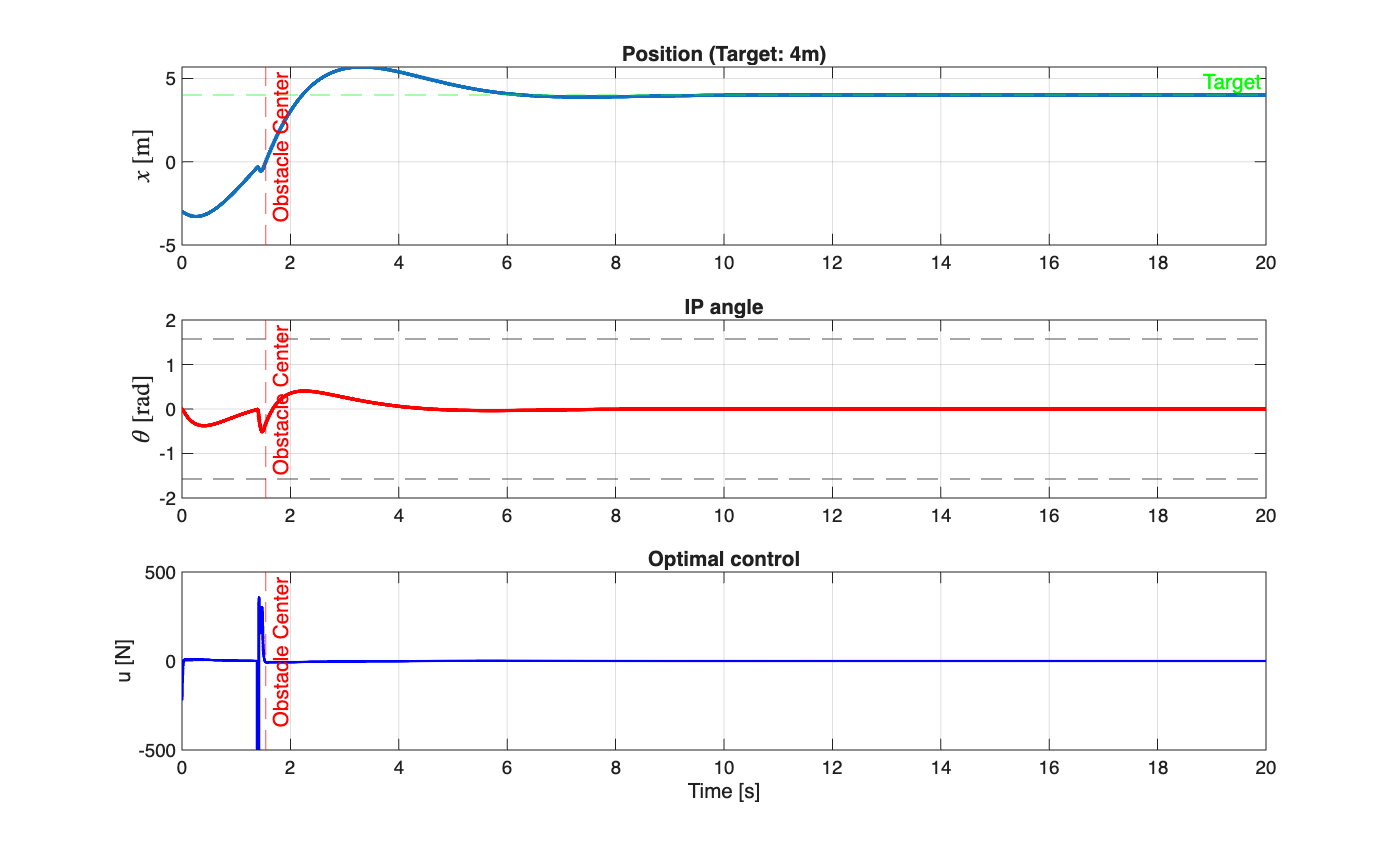
\includegraphics[width=\textwidth]{Fig1_eu.png}
			\end{subfigure}
			\hfill
			\begin{subfigure}[b]{0.48\textwidth}
				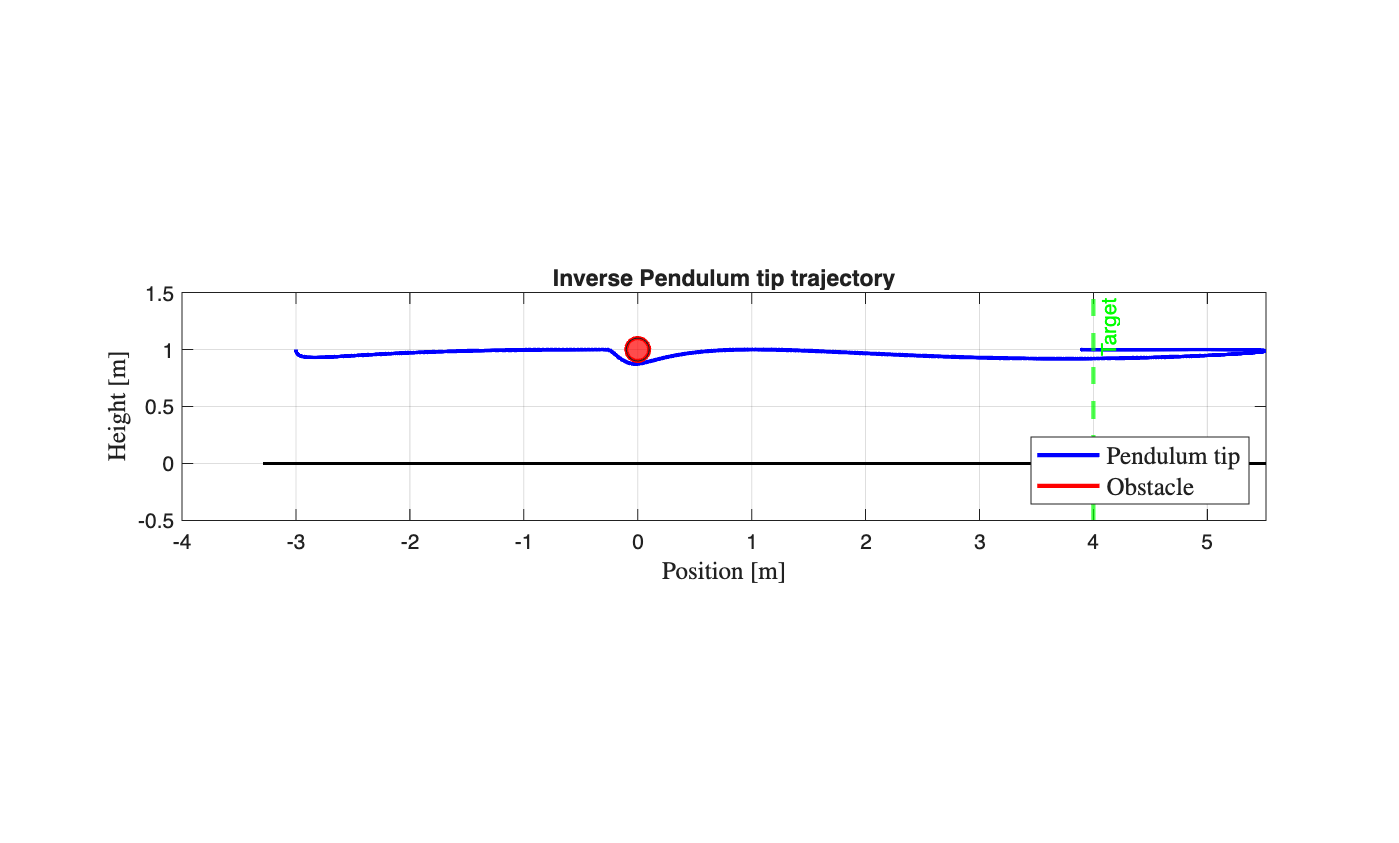
\includegraphics[width=\textwidth]{Fig2_eu.png}
			\end{subfigure}
			
			\vspace{0.2cm}
			
			\begin{subfigure}[b]{0.48\textwidth}
				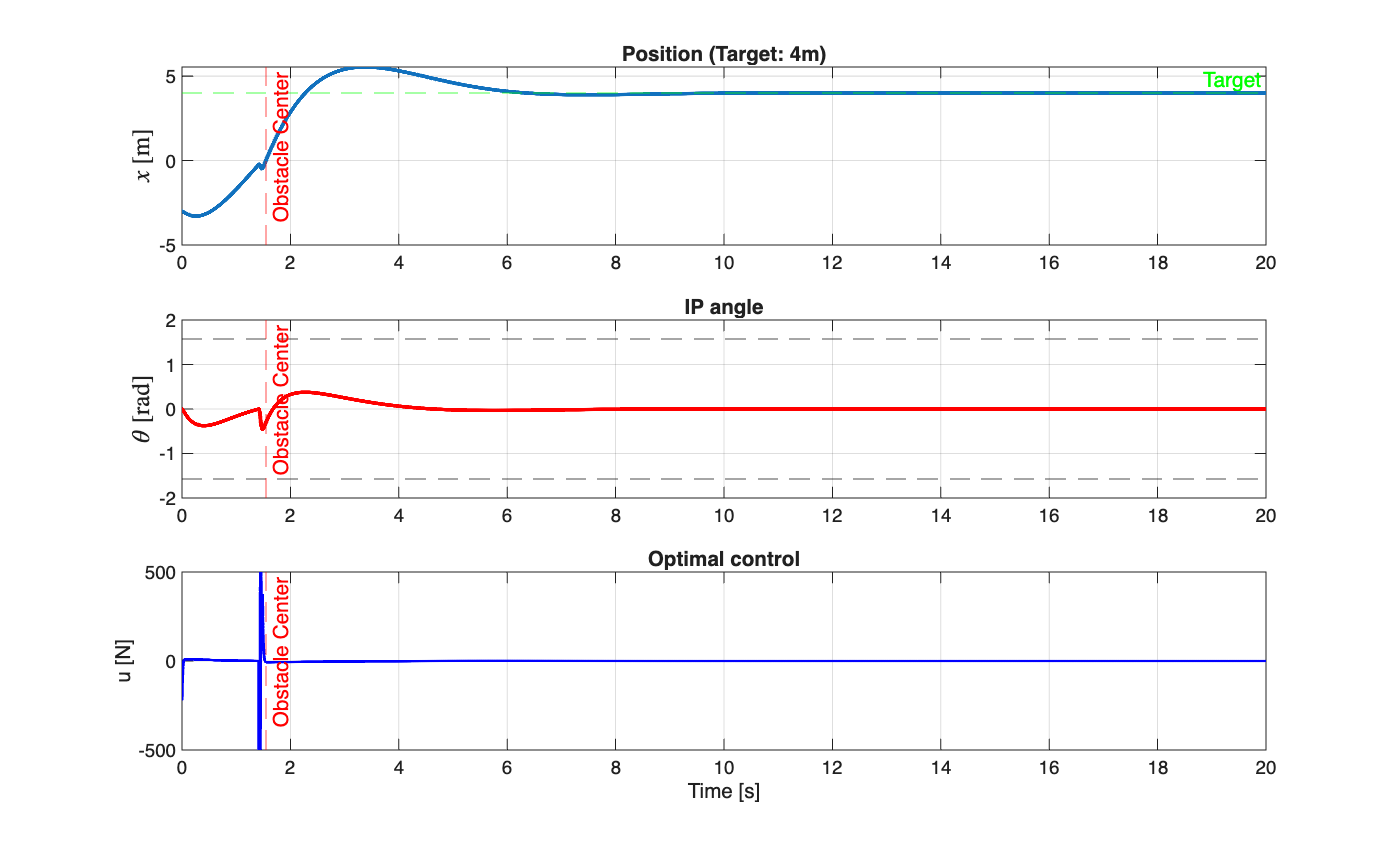
\includegraphics[width=\textwidth]{Fig1_rk.png}
			\end{subfigure}
			\hfill
			\begin{minipage}[b]{0.48\textwidth}
				\centering
			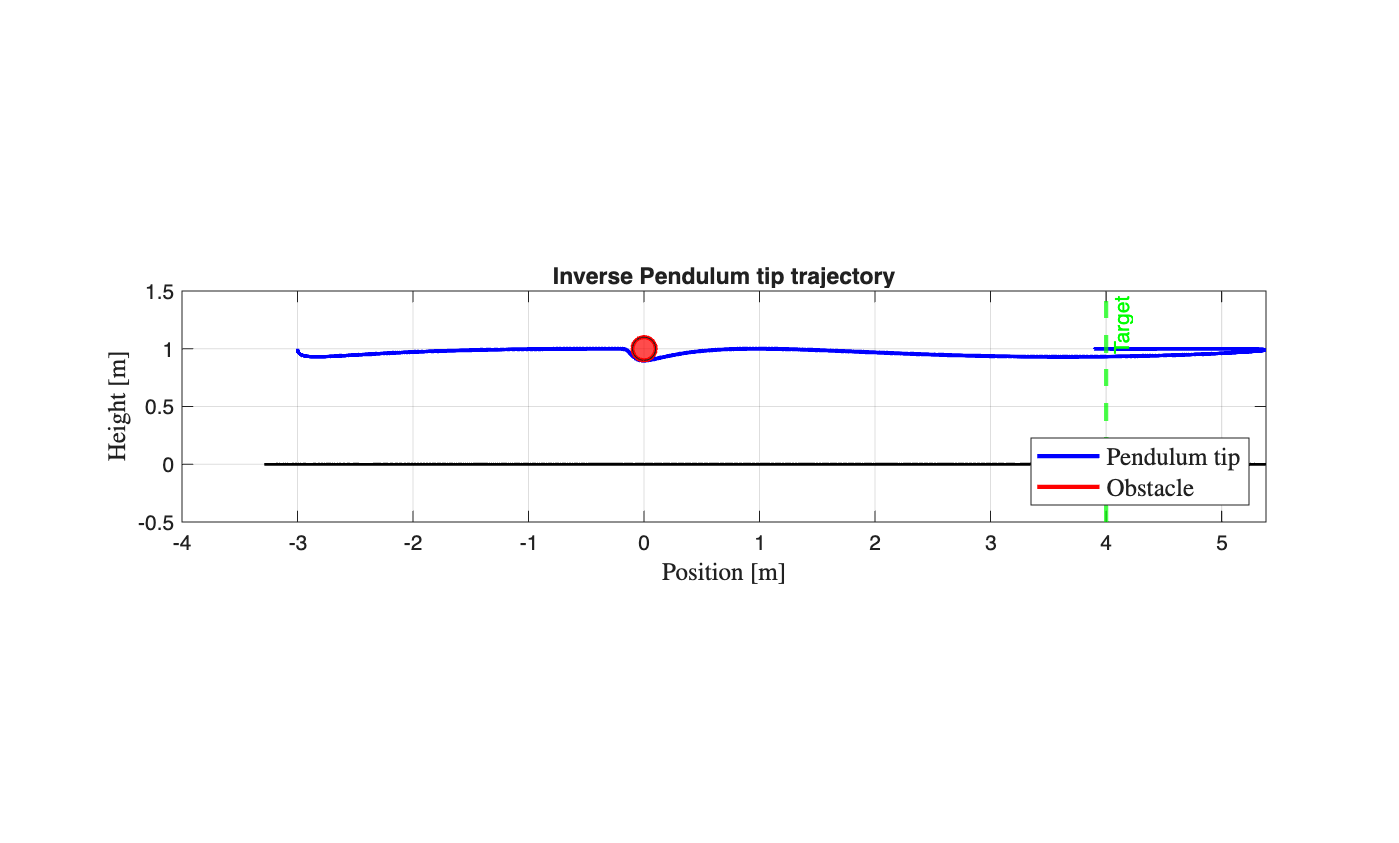
\includegraphics[width=\textwidth]{Fig2_rk.png}
			\end{minipage}
		\end{figure}
	\end{frame}
	
	% Slide 2: Gruppo _2
	\begin{frame}{Risultati Simulazione - Set 2  - 500N}
		\begin{figure}
			\centering
			\begin{subfigure}[b]{0.48\textwidth}
				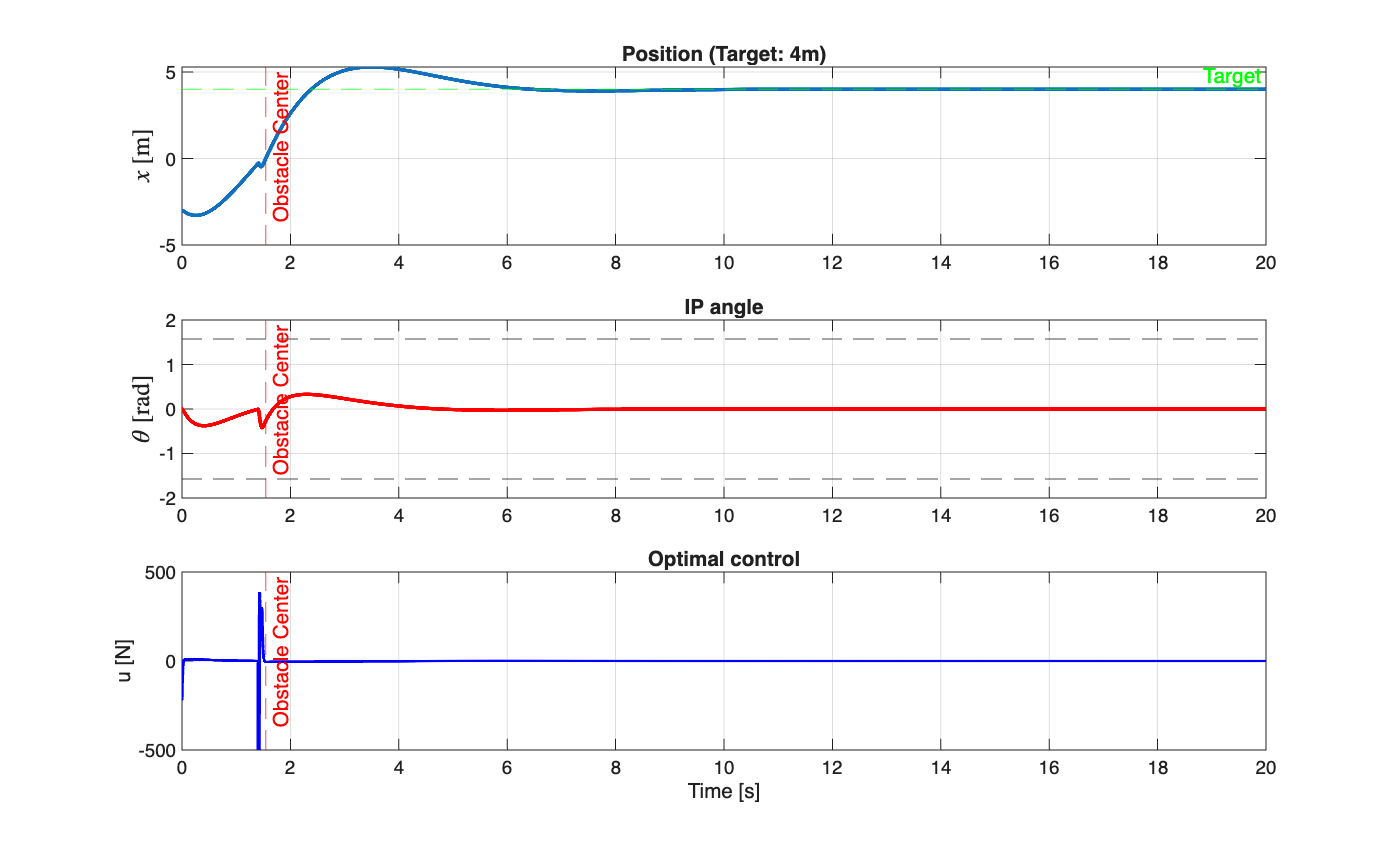
\includegraphics[width=\textwidth]{Fig1_eu_1.png}
		
			\end{subfigure}
			\hfill
			\begin{subfigure}[b]{0.48\textwidth}
				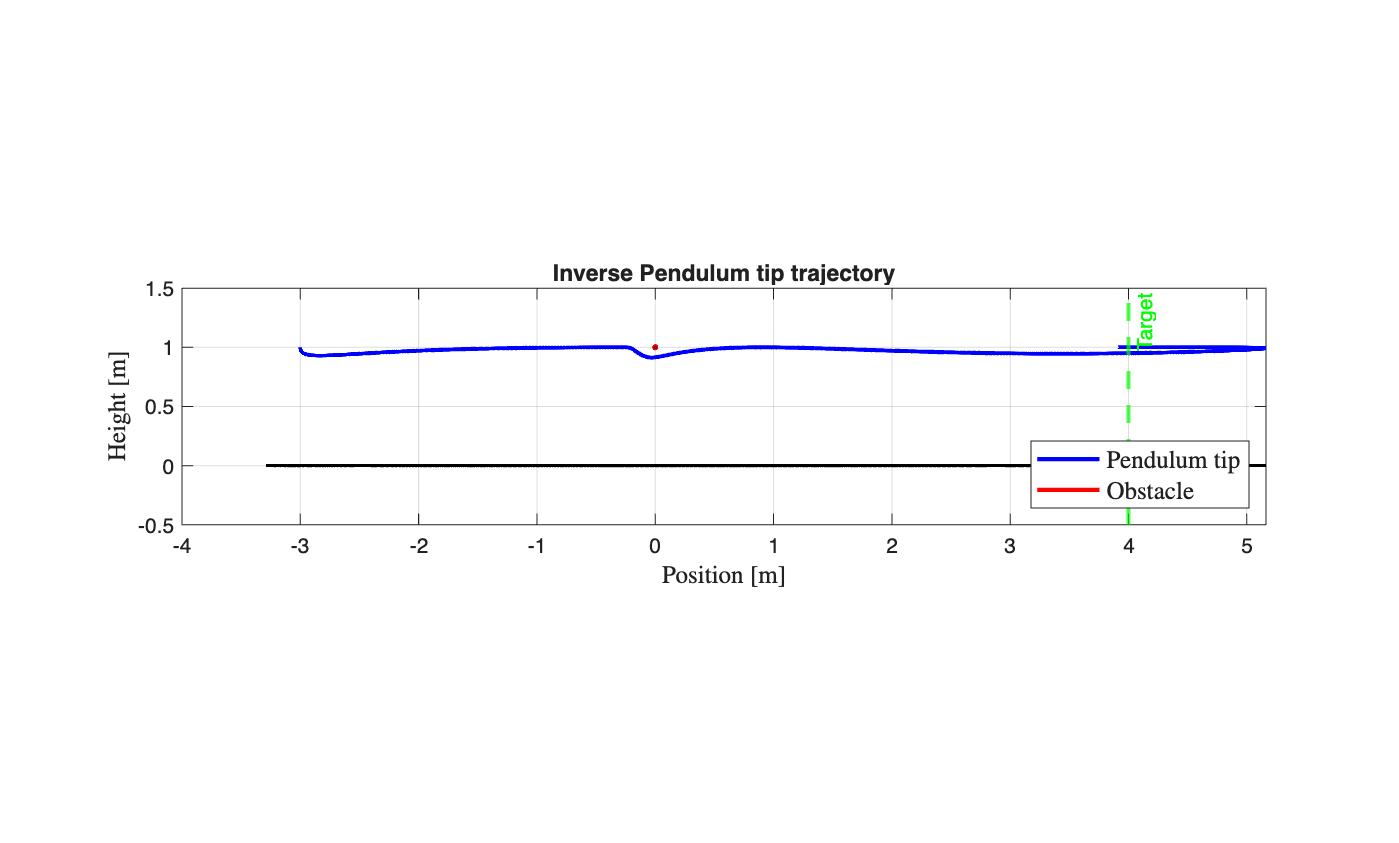
\includegraphics[width=\textwidth]{Fig2_eu_1.png}
		
			\end{subfigure}
			
			\vspace{0.2cm}
			
			\begin{subfigure}[b]{0.48\textwidth}
				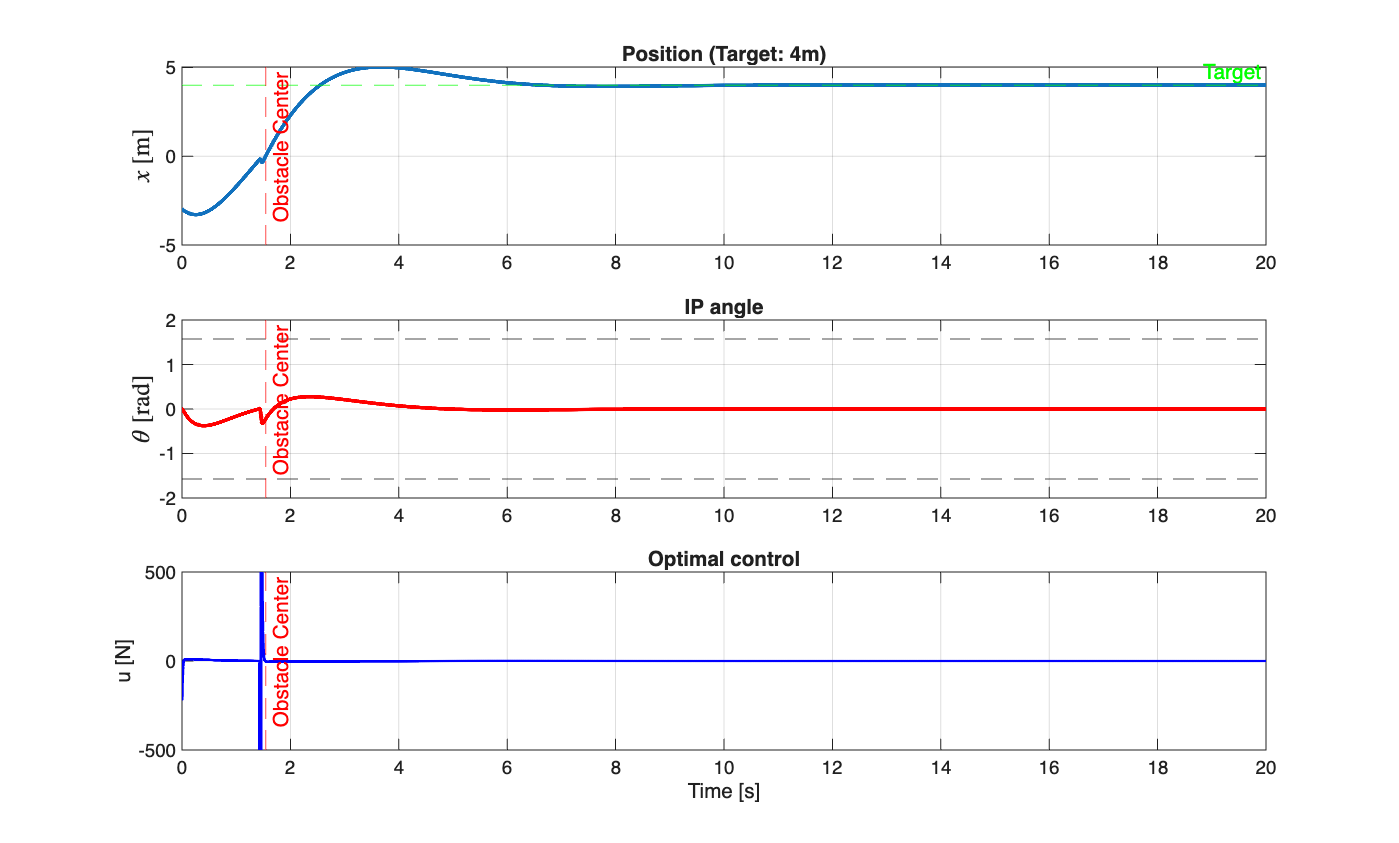
\includegraphics[width=\textwidth]{Fig1_rk_1.png}
			ì
			\end{subfigure}
			\hfill
			\begin{minipage}[b]{0.48\textwidth}
				\centering
				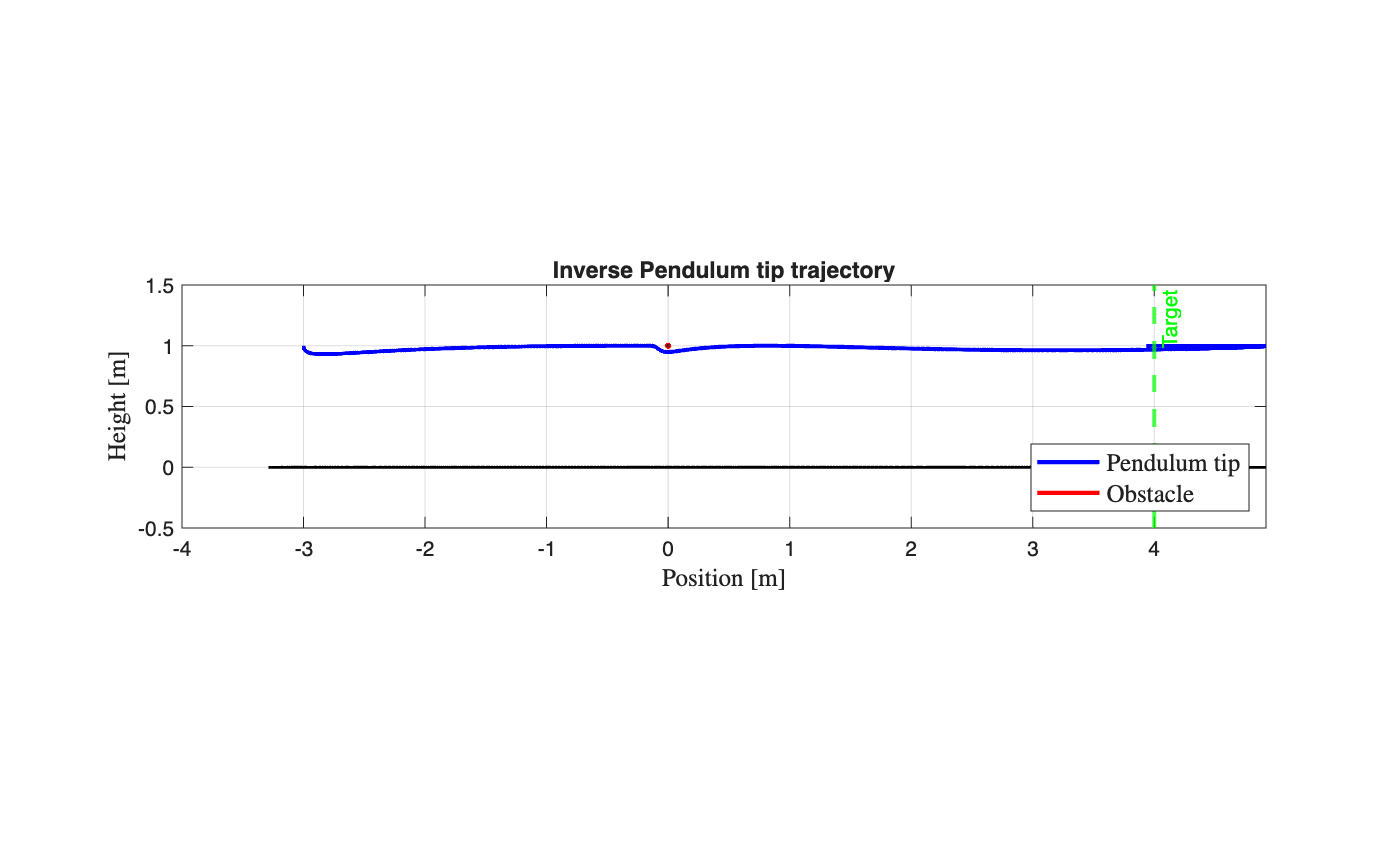
\includegraphics[width=\textwidth]{Fig2_rk_1.png}
			\end{minipage}
		\end{figure}
	\end{frame}
	
	
	% Slide 3: Gruppo _3 e Standard
	\begin{frame}{Risultati Simulazione - Set 3  - 500N}
		\begin{figure}
			\centering
			\begin{subfigure}[b]{0.48\textwidth}
				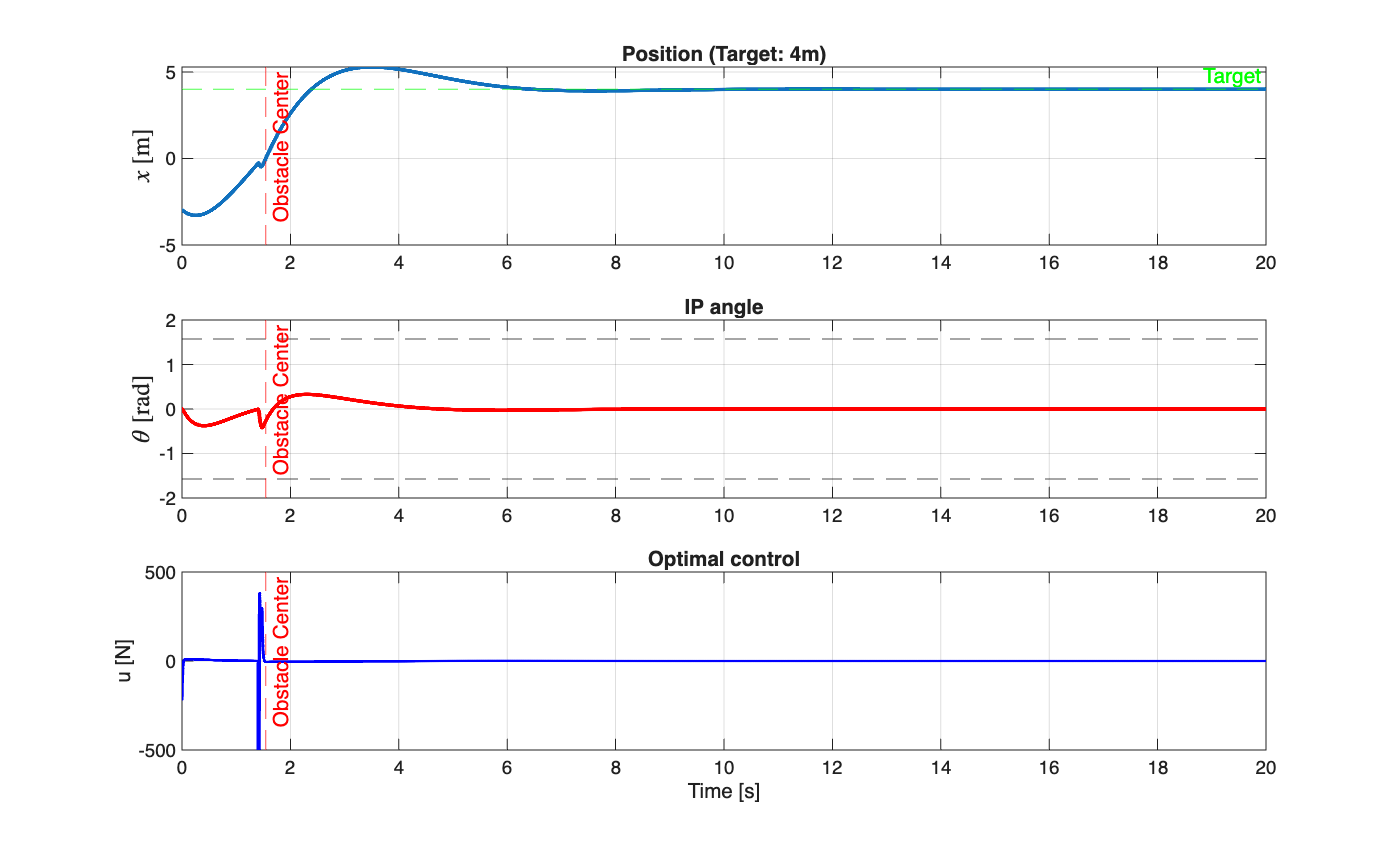
\includegraphics[width=\textwidth]{Fig1_eu_2.png}
				
			\end{subfigure}
			\hfill
			\begin{subfigure}[b]{0.48\textwidth}
				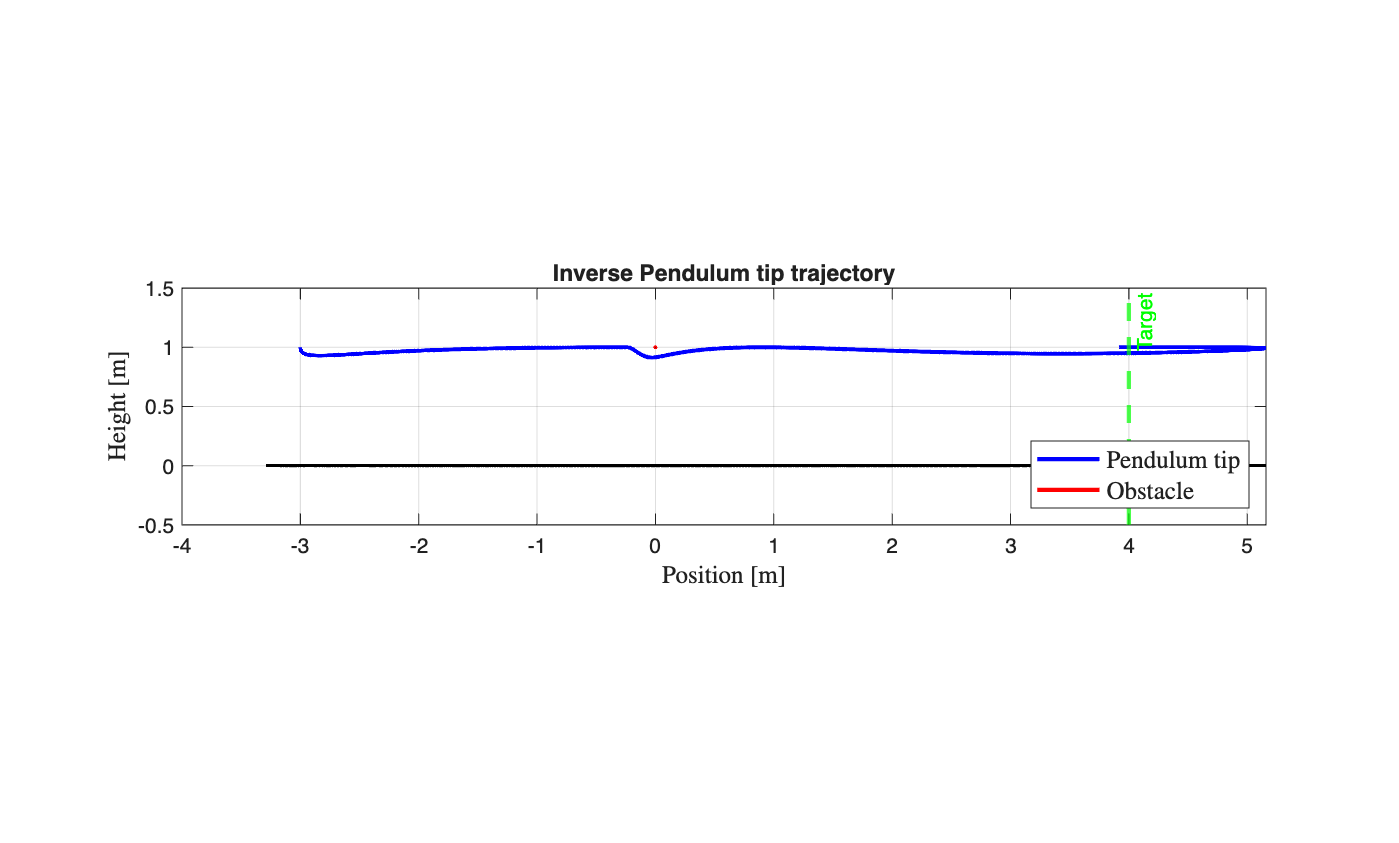
\includegraphics[width=\textwidth]{Fig2_eu_2.png}
			
			\end{subfigure}
			
			\vspace{0.2cm}
			
			\begin{subfigure}[b]{0.48\textwidth}
				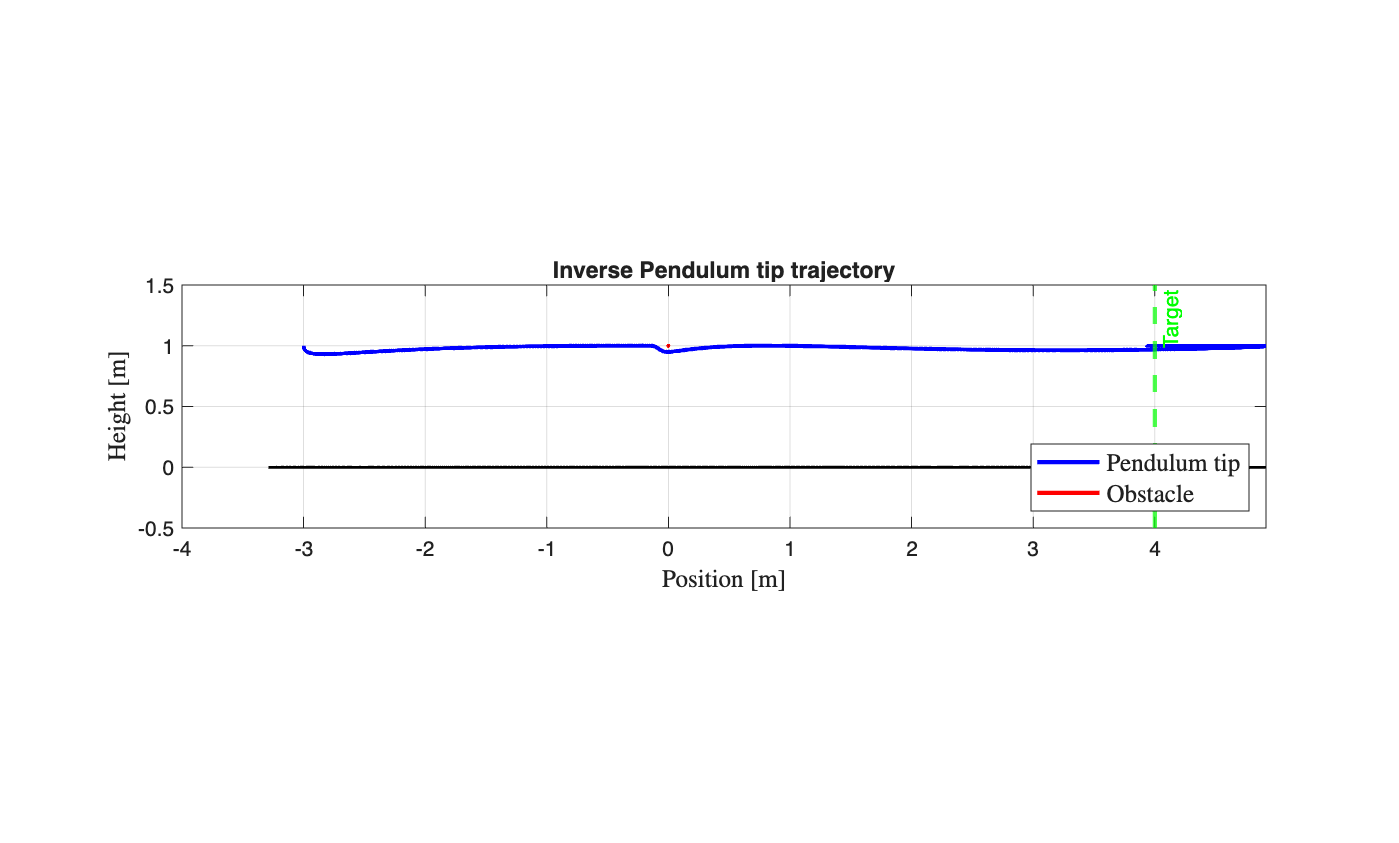
\includegraphics[width=\textwidth]{Fig2_rk_2.png}
			\end{subfigure}
			\hfill
			\begin{subfigure}[b]{0.48\textwidth}
				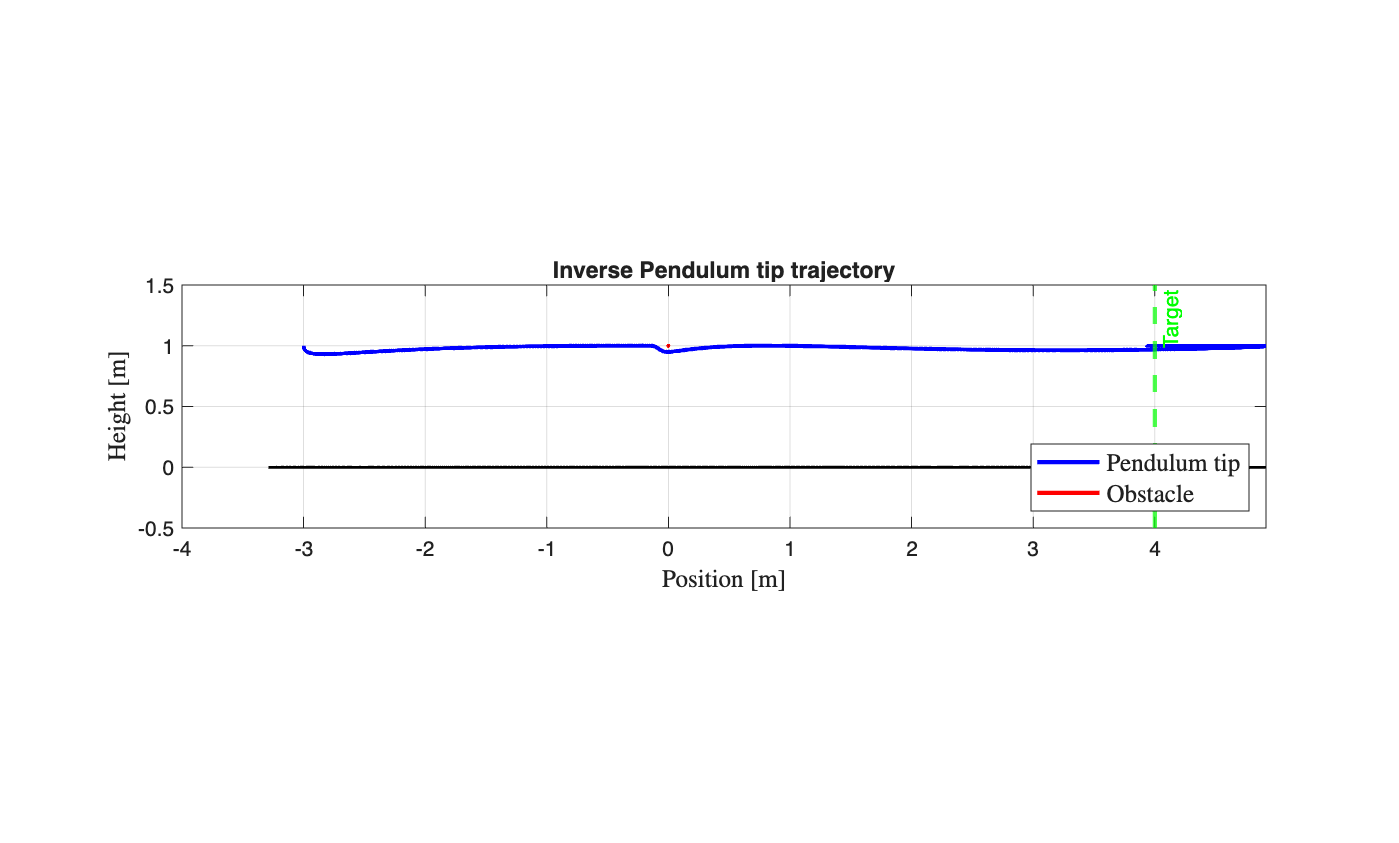
\includegraphics[width=\textwidth]{Fig2_rk_2.png}
			\end{subfigure}
		\end{figure}
	\end{frame}
	
	% Slide 3: Gruppo _3 e Standard
	\begin{frame}{Risultati Simulazione - Set 4 - 500N}
		\begin{figure}
			\centering
			\begin{subfigure}[b]{0.48\textwidth}
				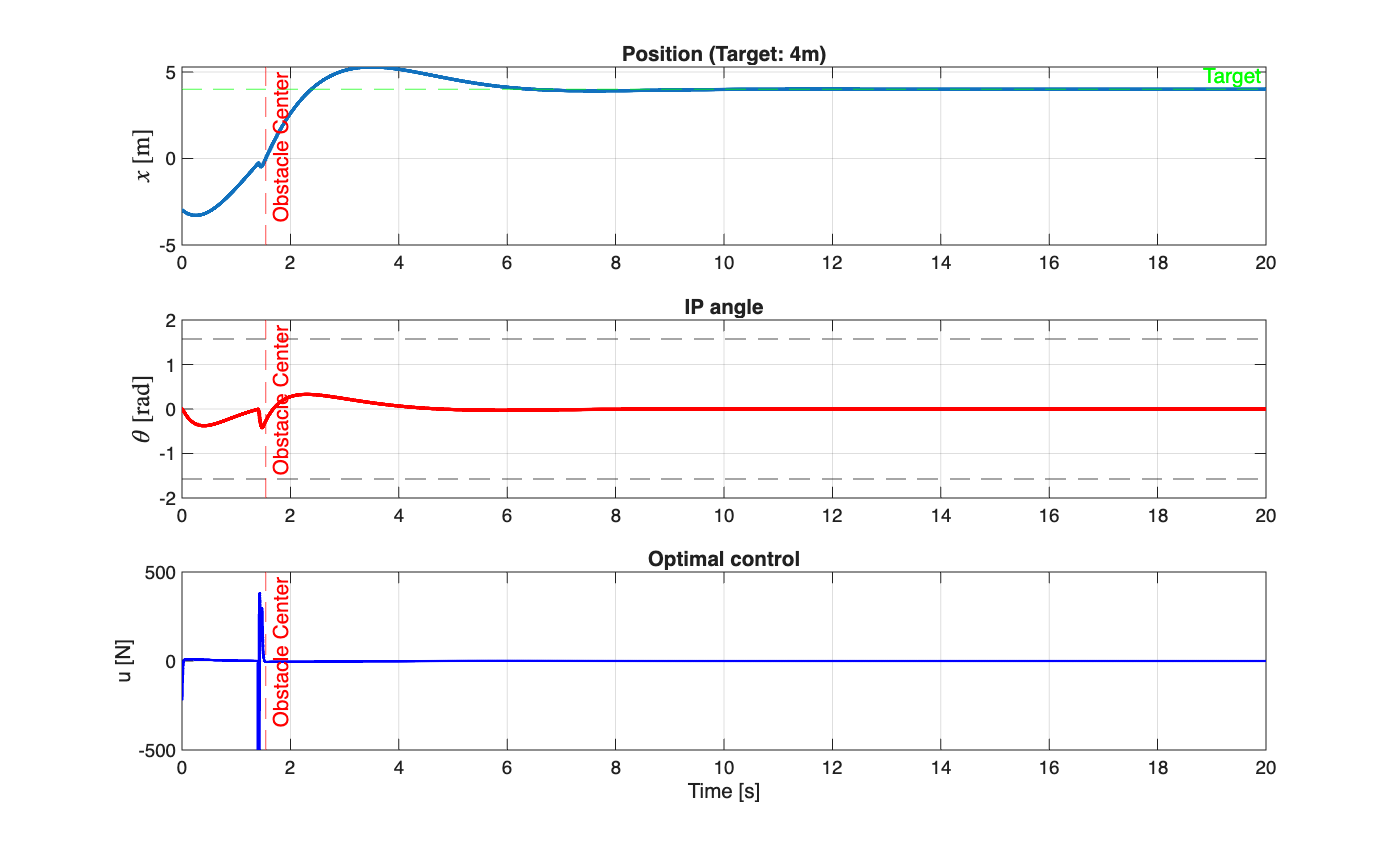
\includegraphics[width=\textwidth]{Fig1_eu_3.png}
		
			\end{subfigure}
			\hfill
			\begin{subfigure}[b]{0.48\textwidth}
				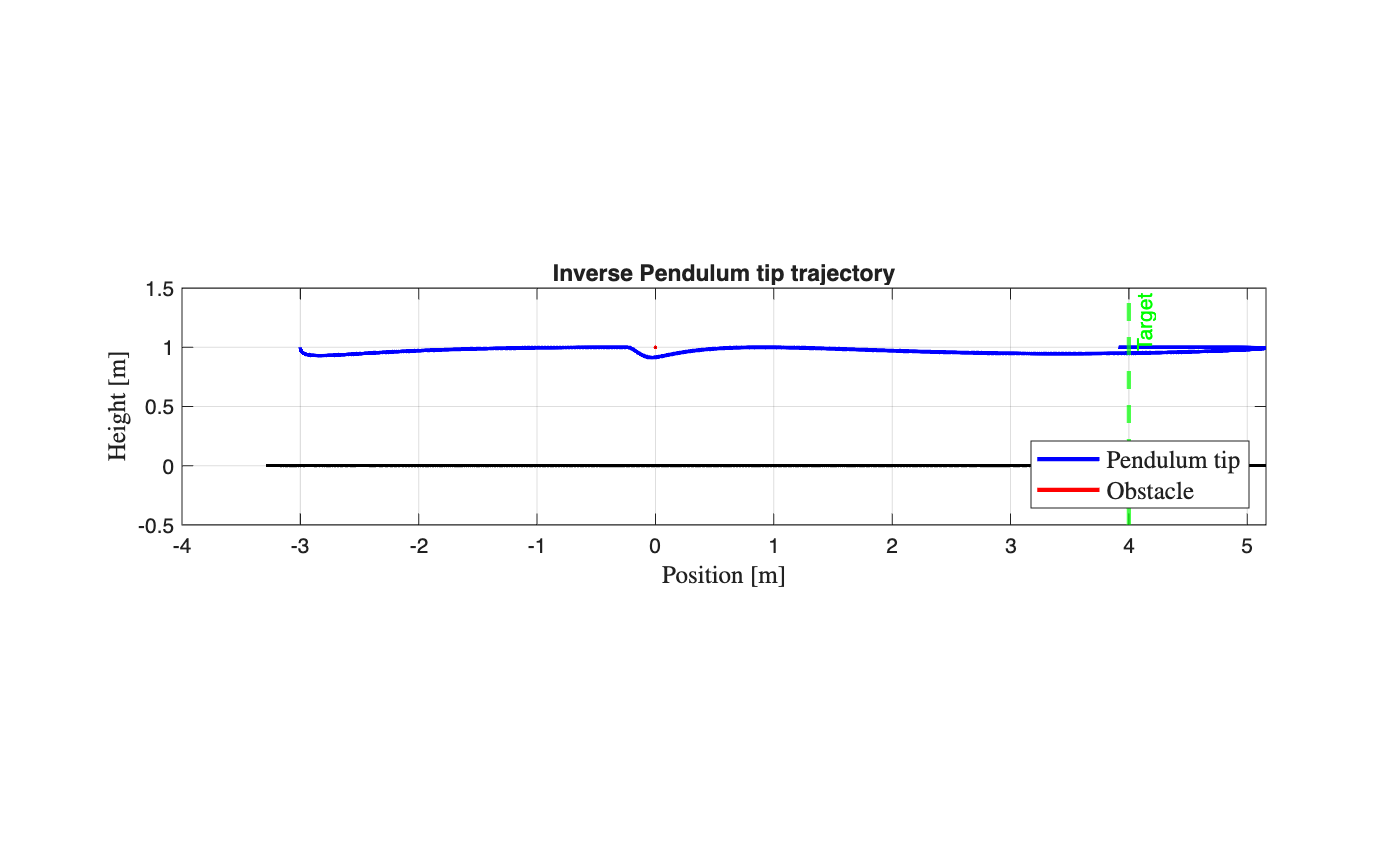
\includegraphics[width=\textwidth]{Fig2_eu_3.png}
			
			\end{subfigure}
			
			\vspace{0.2cm}
			
			\begin{subfigure}[b]{0.48\textwidth}
				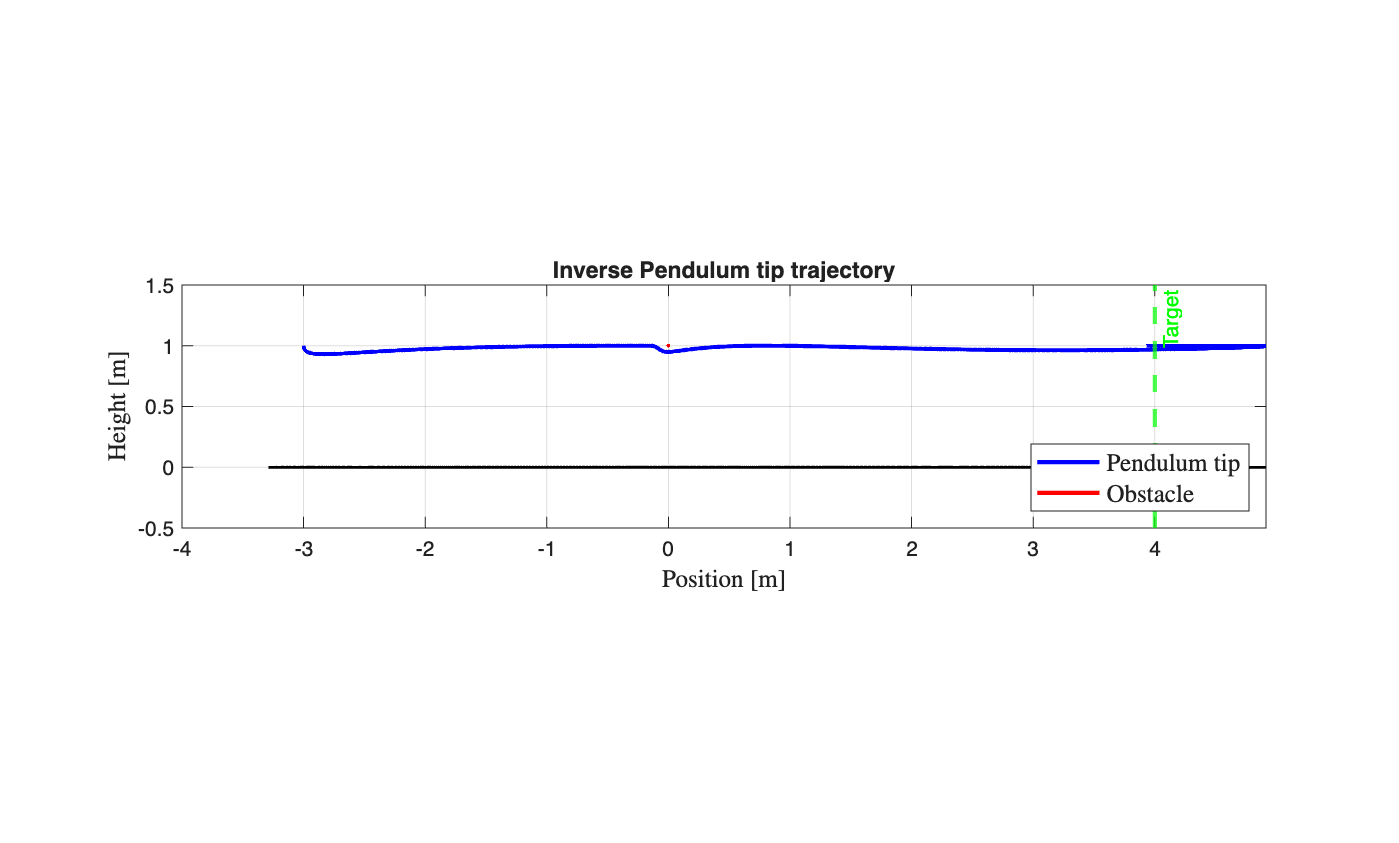
\includegraphics[width=\textwidth]{Fig2_rk_3.png}
			\end{subfigure}
			\hfill
			\begin{subfigure}[b]{0.48\textwidth}
				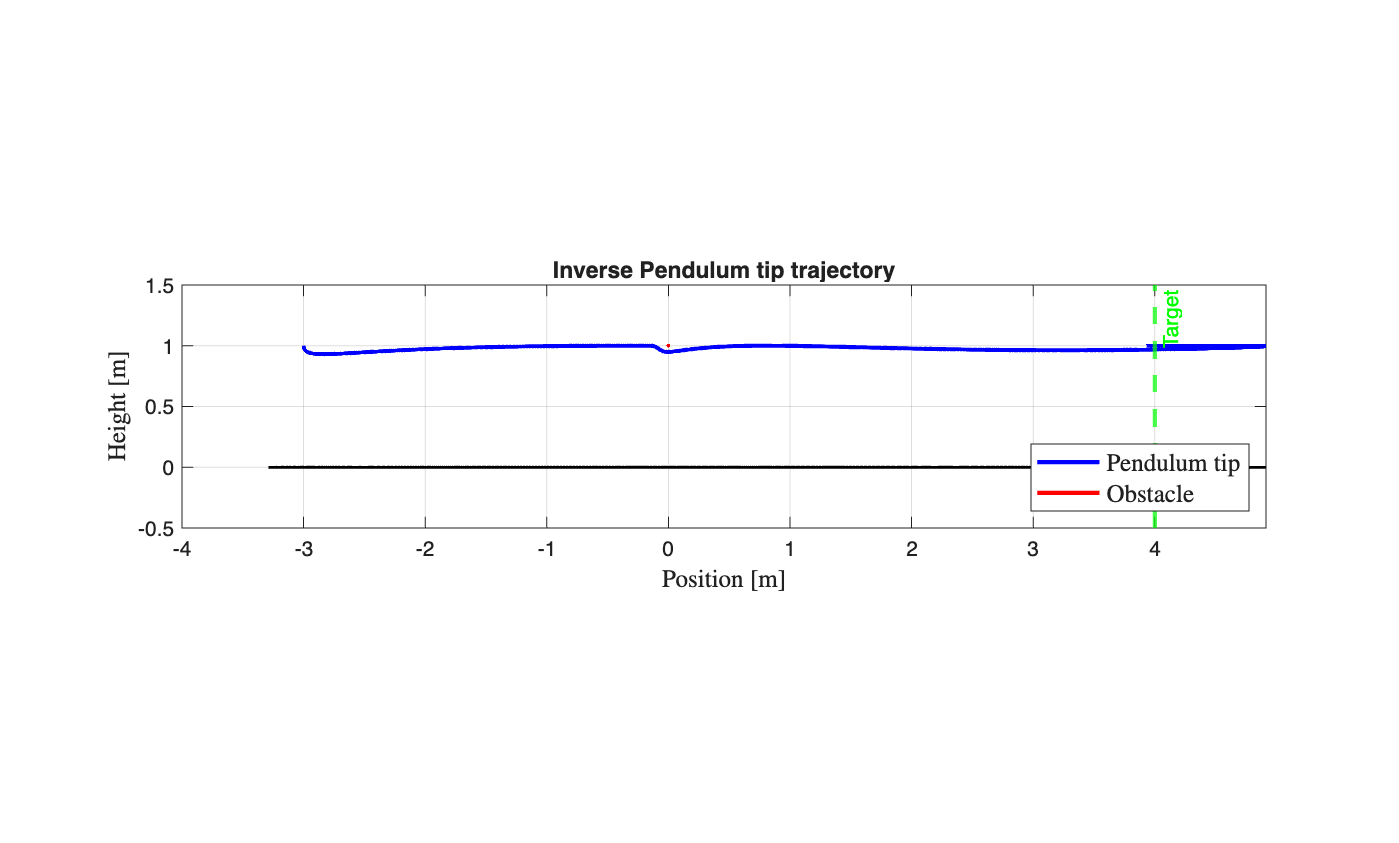
\includegraphics[width=\textwidth]{Fig2_rk_3.png}
			\end{subfigure}
		\end{figure}
	\end{frame}
	
	\begin{frame}{Risultati Simulazione - Set 5  - 500N }
	\begin{figure}
		\centering
		\begin{subfigure}[b]{0.48\textwidth}
			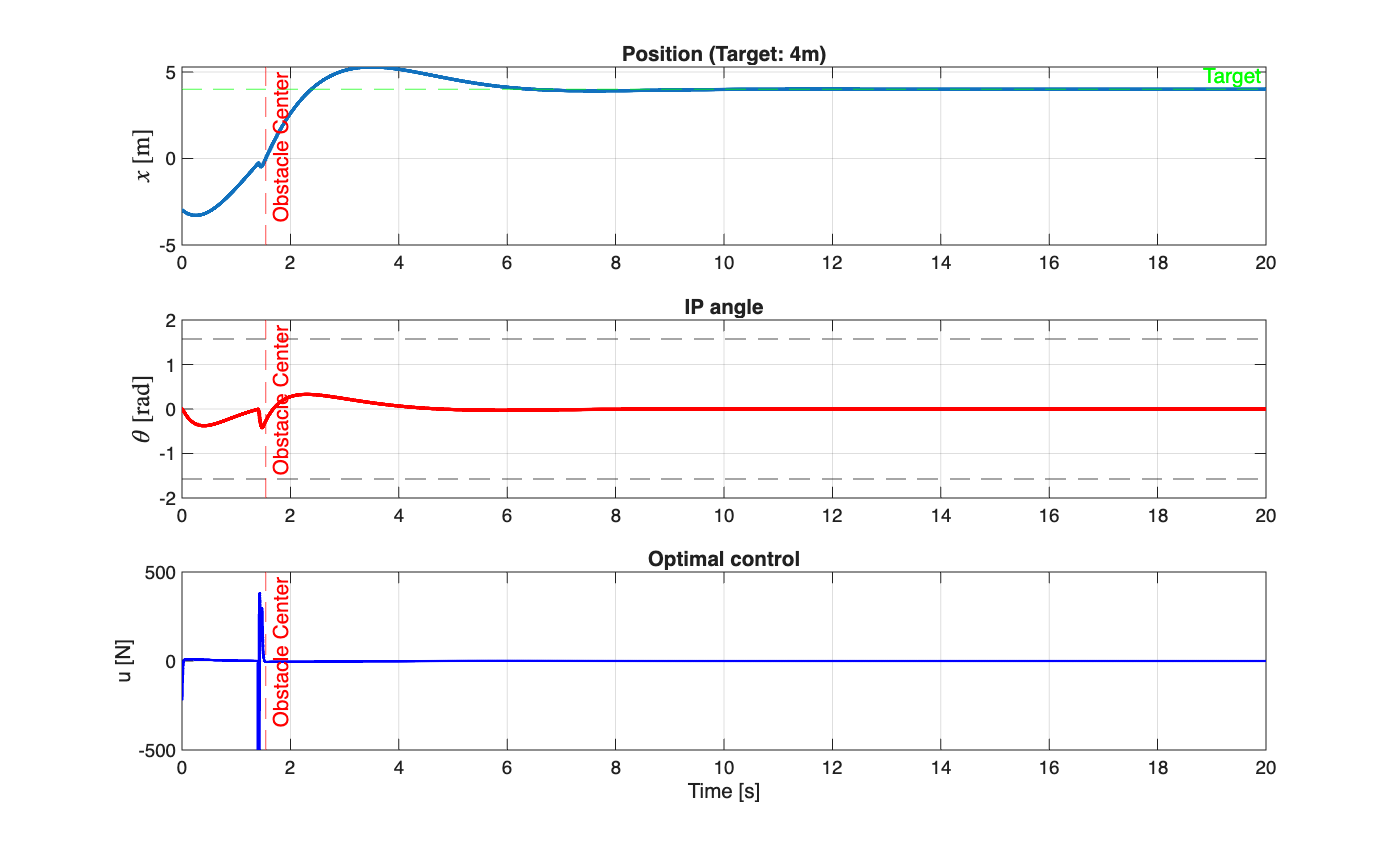
\includegraphics[width=\textwidth]{Fig1_eu_3.png}
			
		\end{subfigure}
		\hfill
		\begin{subfigure}[b]{0.48\textwidth}
			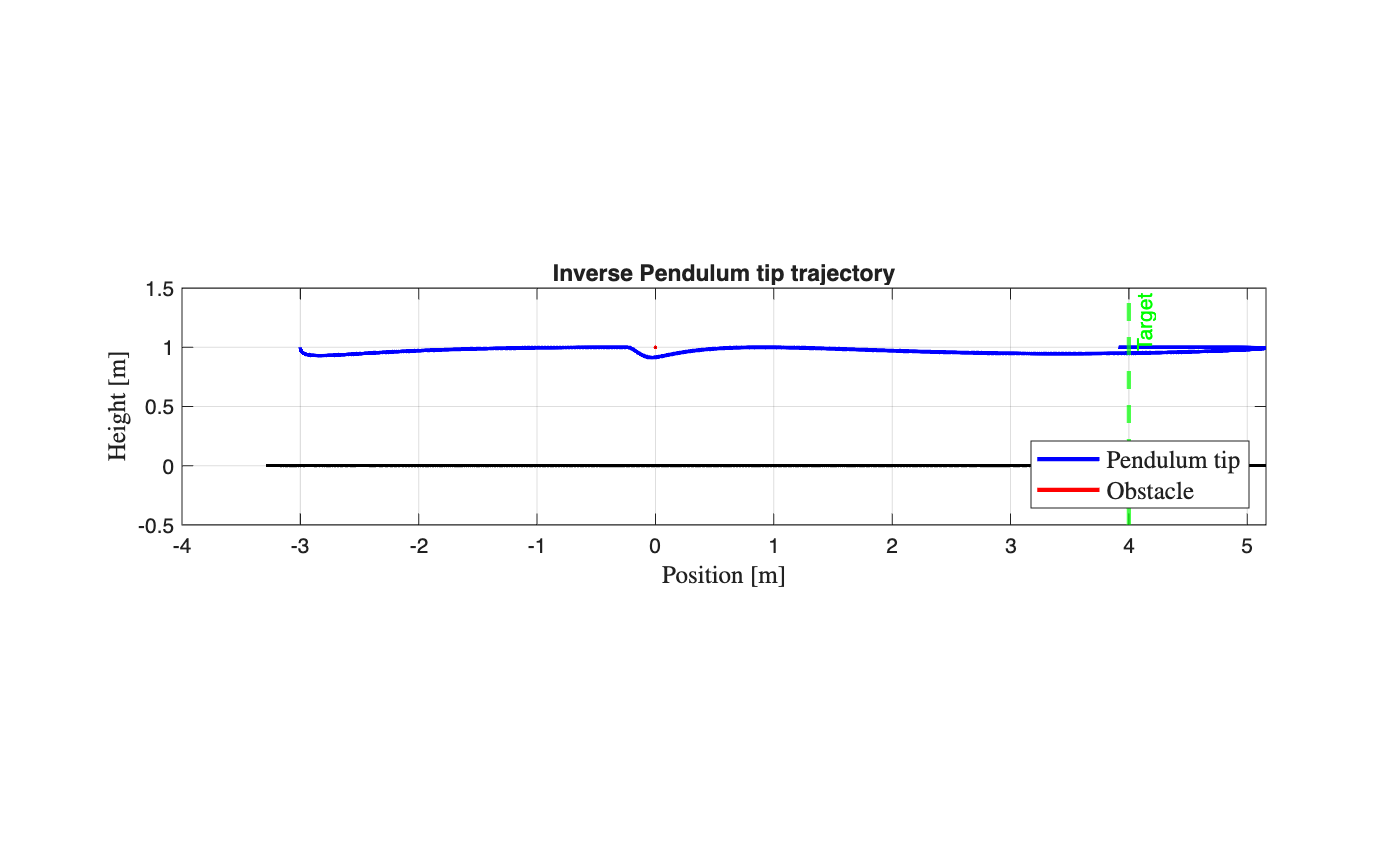
\includegraphics[width=\textwidth]{Fig2_eu_3.png}
			
		\end{subfigure}
		
		\vspace{0.2cm}
		
		\begin{subfigure}[b]{0.48\textwidth}
			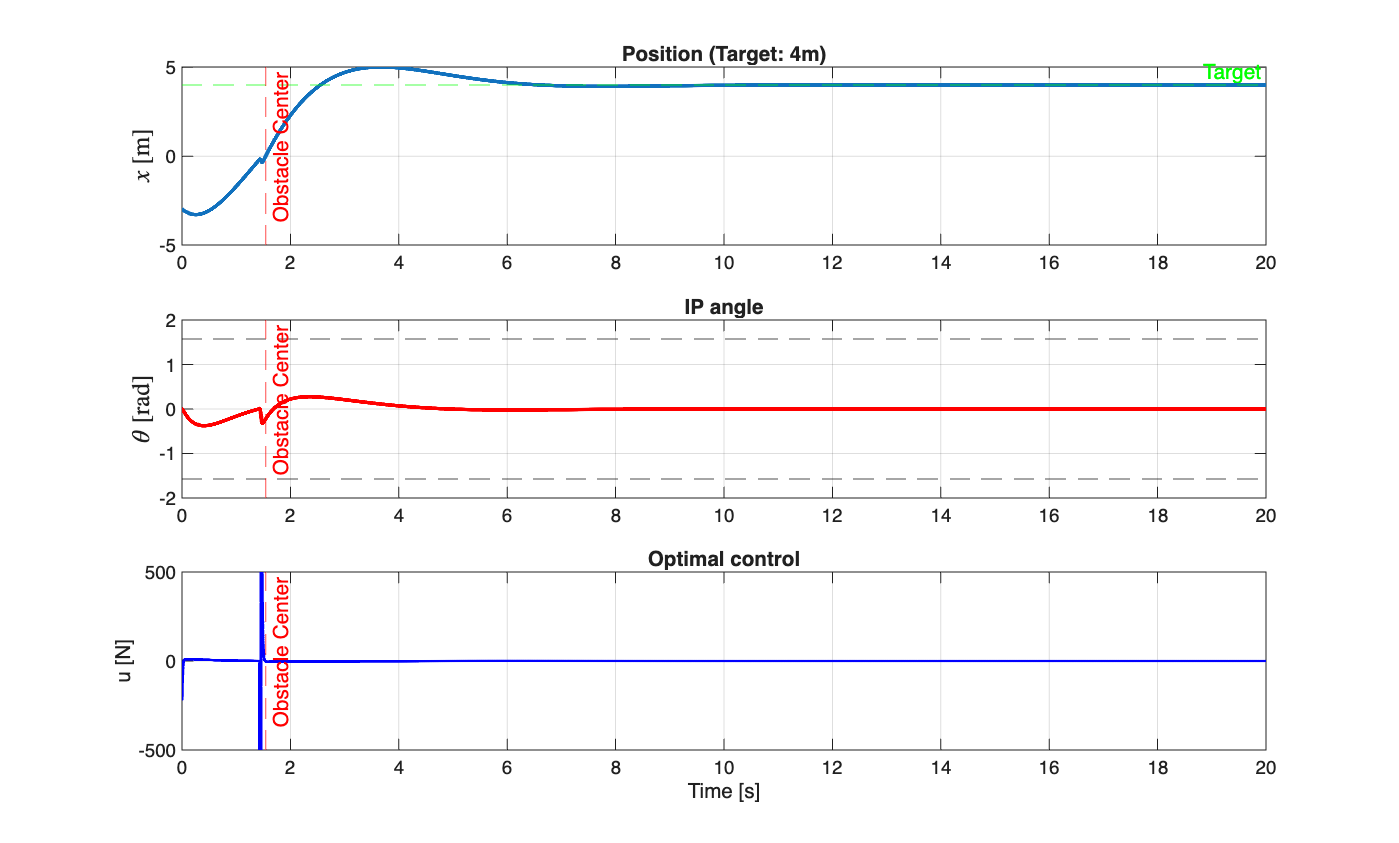
\includegraphics[width=\textwidth]{Fig1_rk_3.png}
		\end{subfigure}
		\hfill
		\begin{subfigure}[b]{0.48\textwidth}
			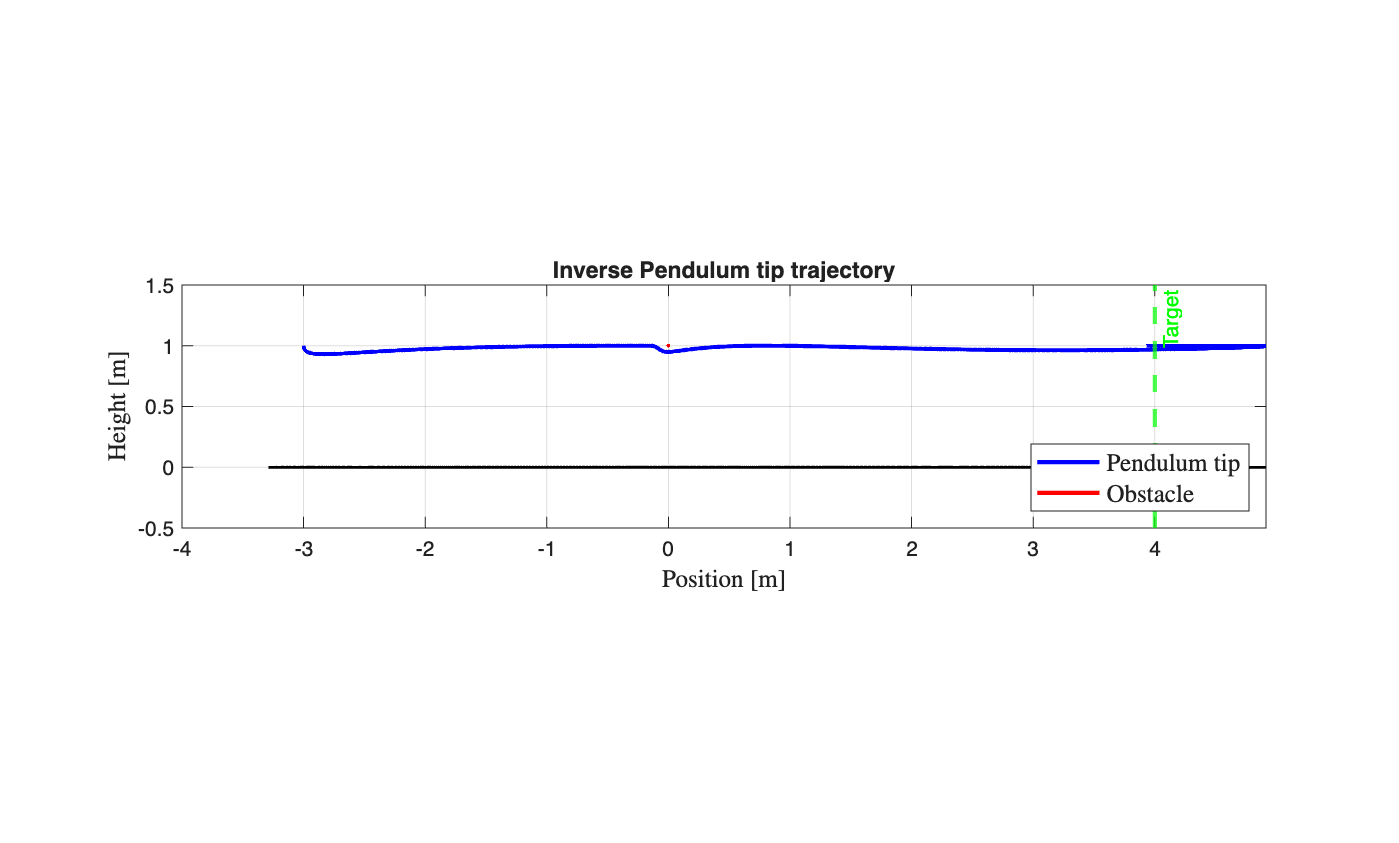
\includegraphics[width=\textwidth]{Fig2_rk_3.png}
		\end{subfigure}
	\end{figure}
\end{frame}	


	\begin{frame}{Risultati Simulazione - Set 1 - INF}
	\begin{figure}
		\centering
		\begin{subfigure}[b]{0.48\textwidth}
			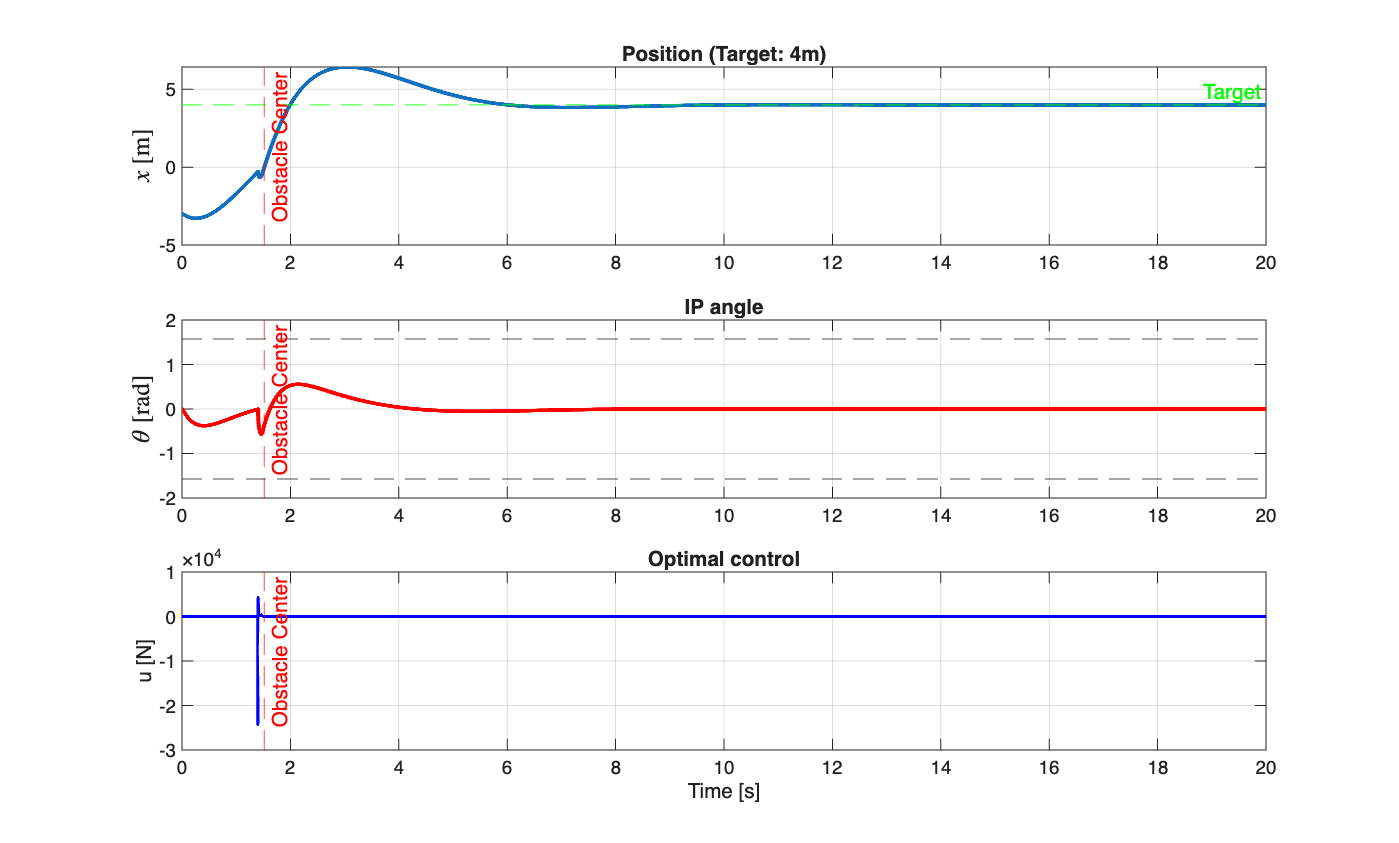
\includegraphics[width=\textwidth]{INF/Fig1_eu_inf.png}
			
		\end{subfigure}
		\hfill
		\begin{subfigure}[b]{0.48\textwidth}
			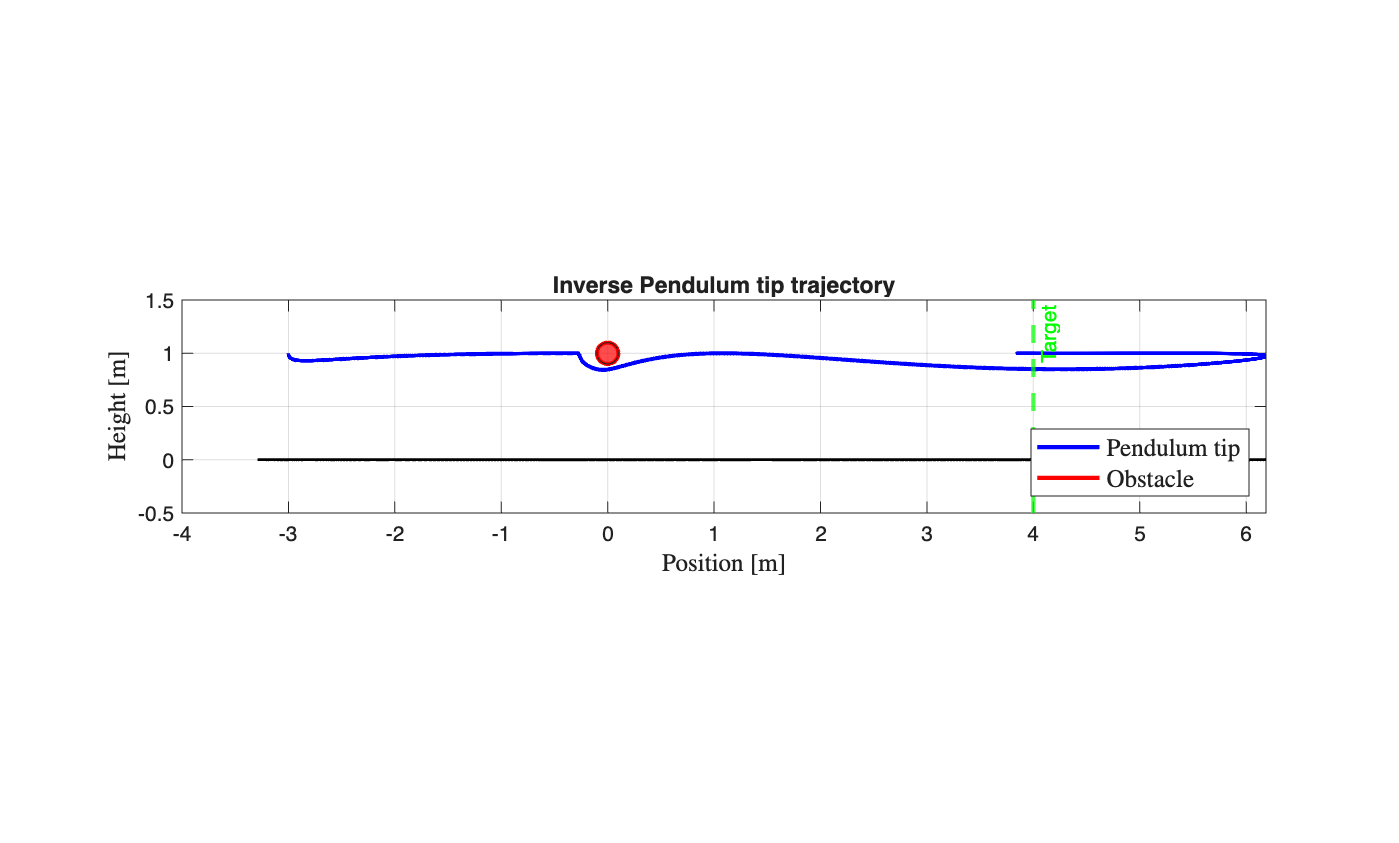
\includegraphics[width=\textwidth]{INF/Fig2_eu_inf.png}
			
		\end{subfigure}
		
		\vspace{0.2cm}
		
		\begin{subfigure}[b]{0.48\textwidth}
			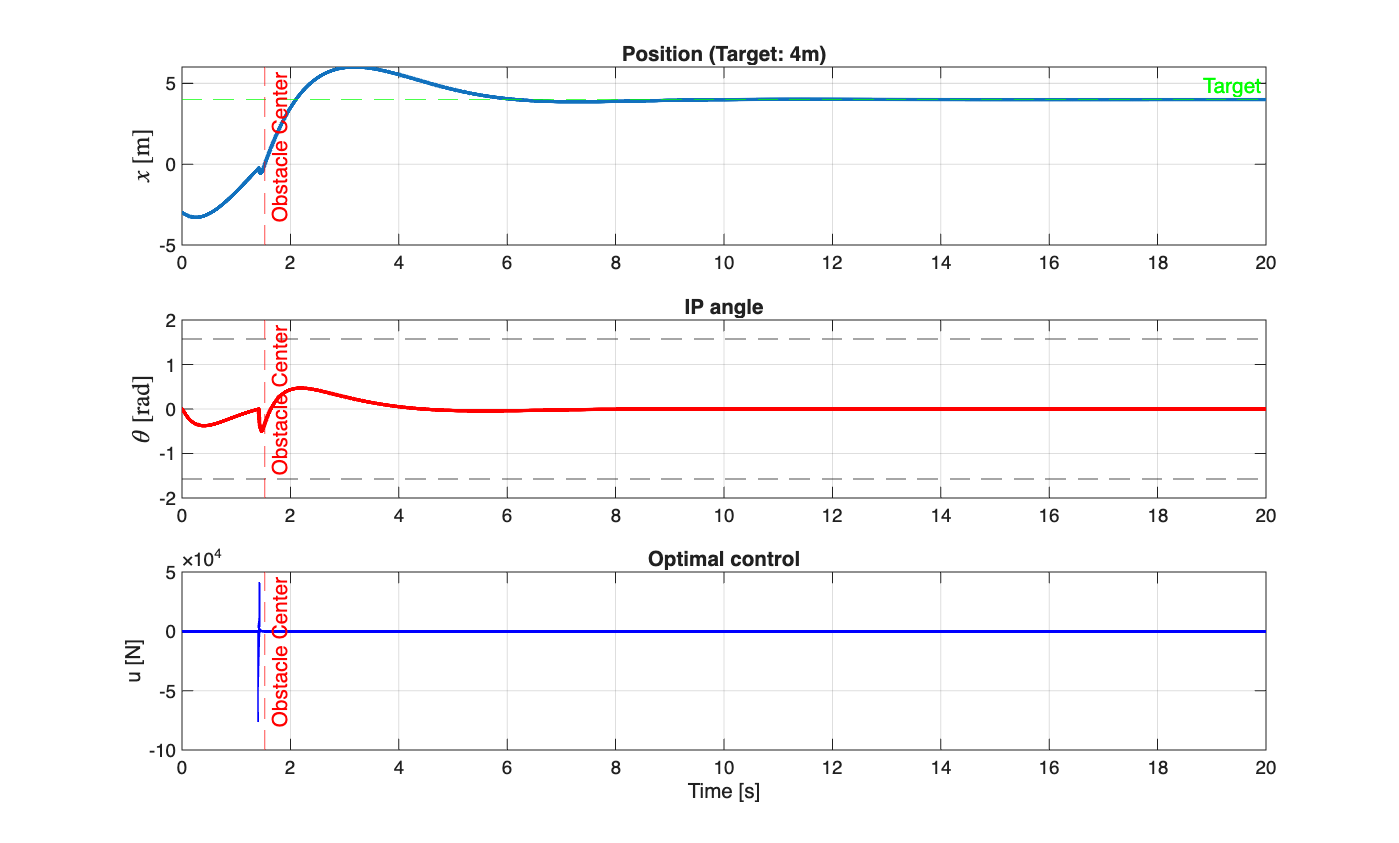
\includegraphics[width=\textwidth]{INF/Fig1_rk_inf.png}
		\end{subfigure}
		\hfill
		\begin{subfigure}[b]{0.48\textwidth}
			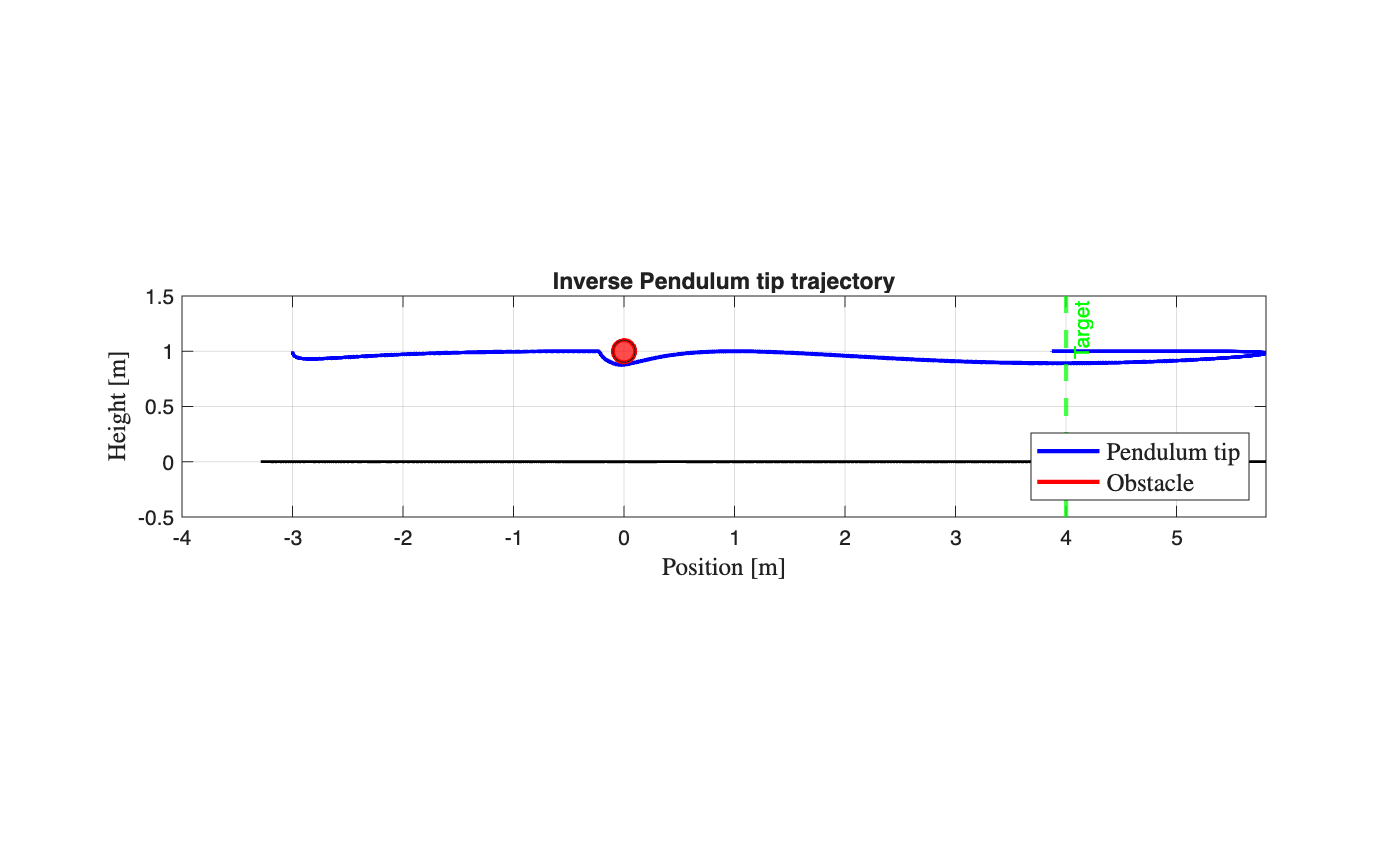
\includegraphics[width=\textwidth]{INF/Fig2_rk_inf.png}
		\end{subfigure}
	\end{figure}
\end{frame}	


	\begin{frame}{Risultati Simulazione - Set 2 - INF }
	\begin{figure}
		\centering
		\begin{subfigure}[b]{0.48\textwidth}
			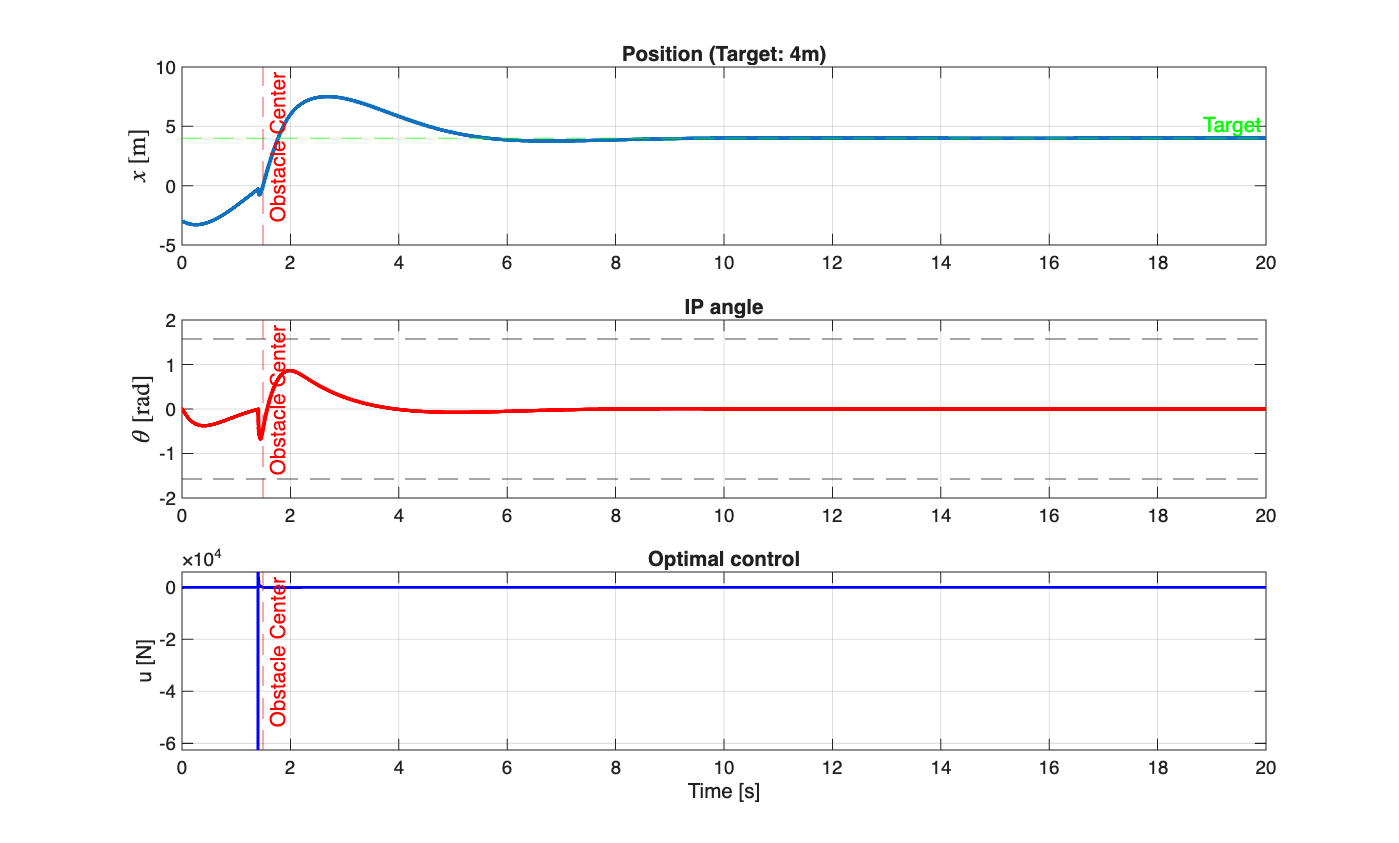
\includegraphics[width=\textwidth]{INF/Fig1_eu_inf_2.png}
			
		\end{subfigure}
		\hfill
		\begin{subfigure}[b]{0.48\textwidth}
			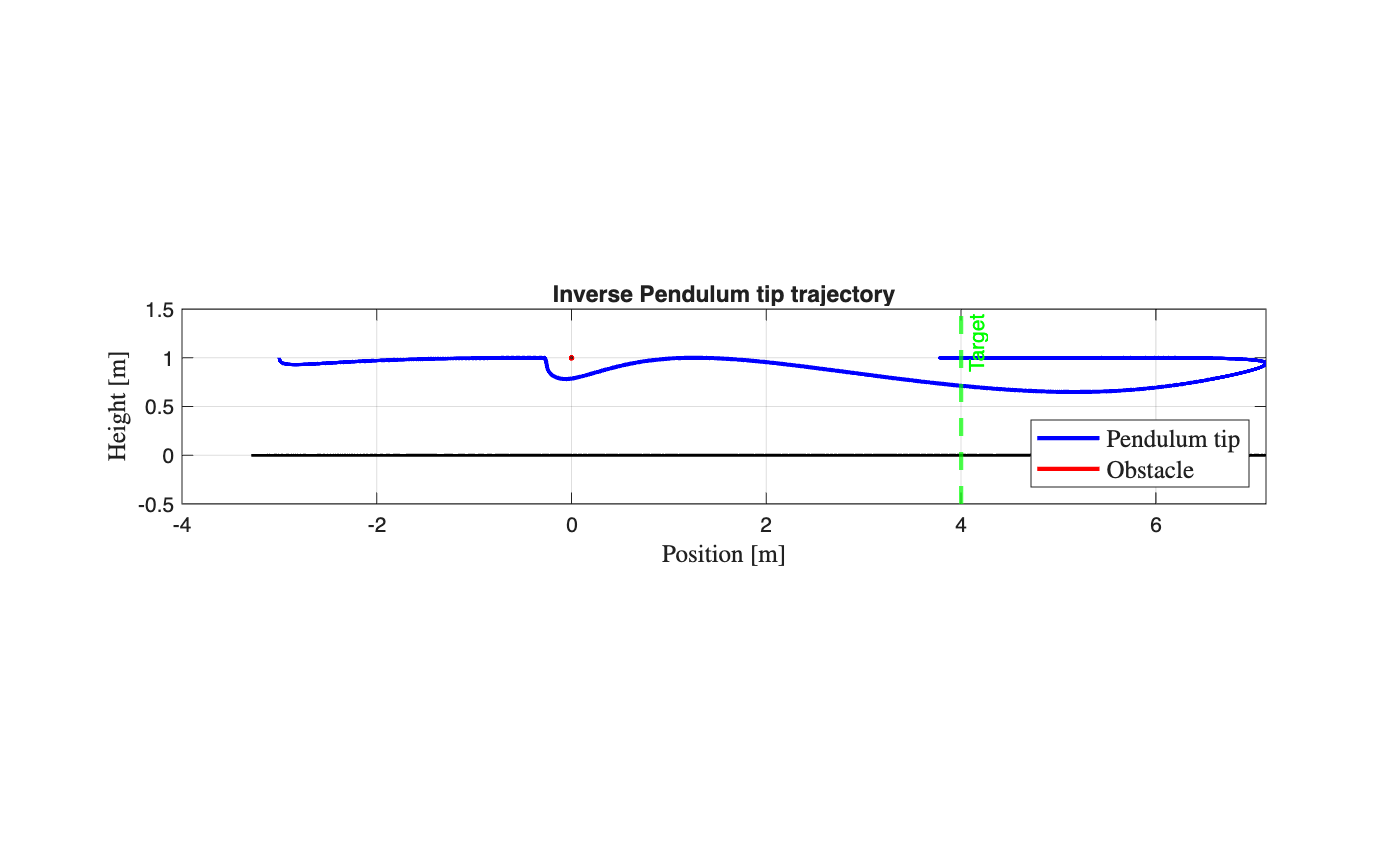
\includegraphics[width=\textwidth]{INF/Fig2_eu_inf_2.png}
			
		\end{subfigure}
		
		\vspace{0.2cm}
		
		\begin{subfigure}[b]{0.48\textwidth}
			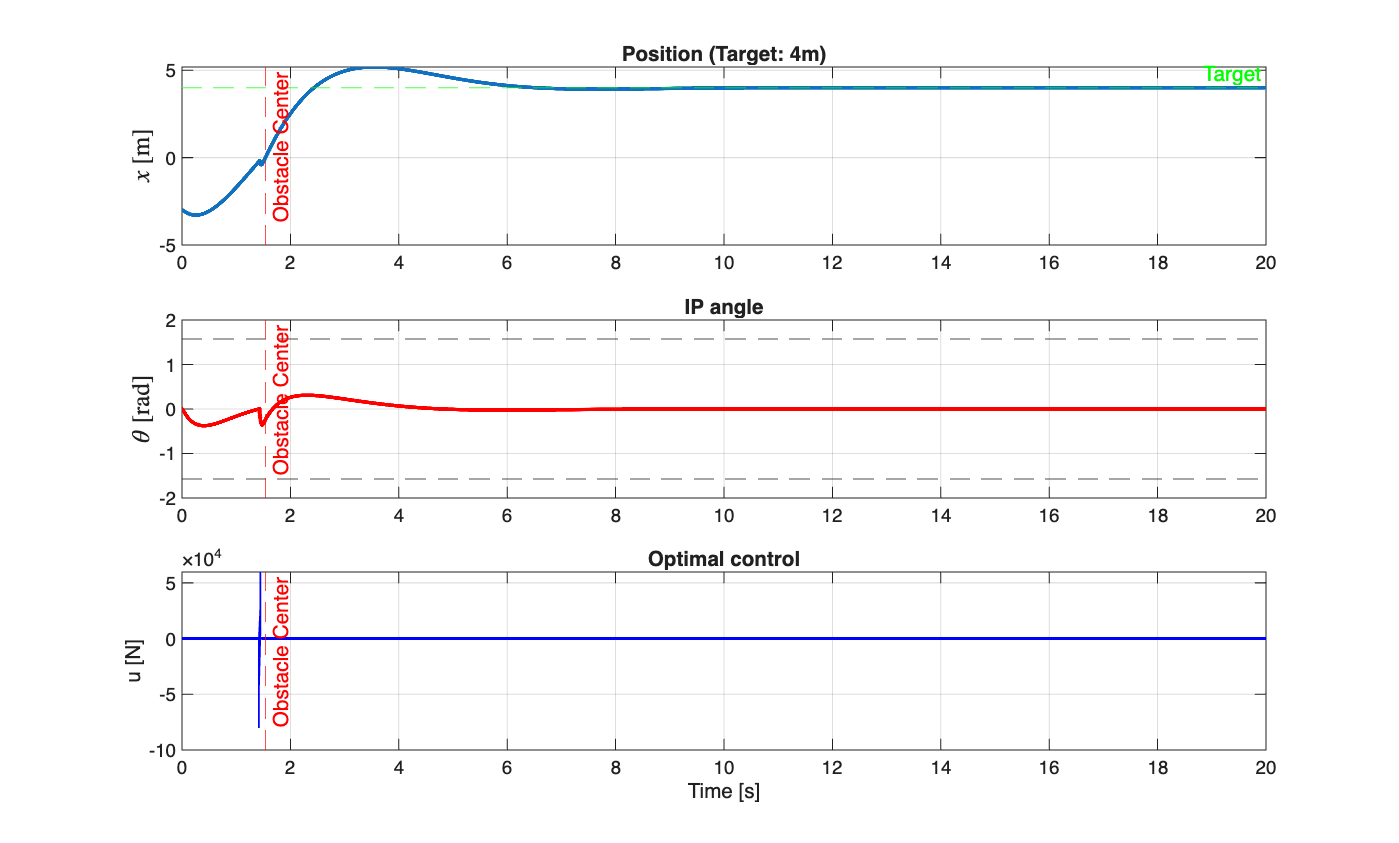
\includegraphics[width=\textwidth]{INF/Fig1_rk_inf_2.png}
		\end{subfigure}
		\hfill
		\begin{subfigure}[b]{0.48\textwidth}
			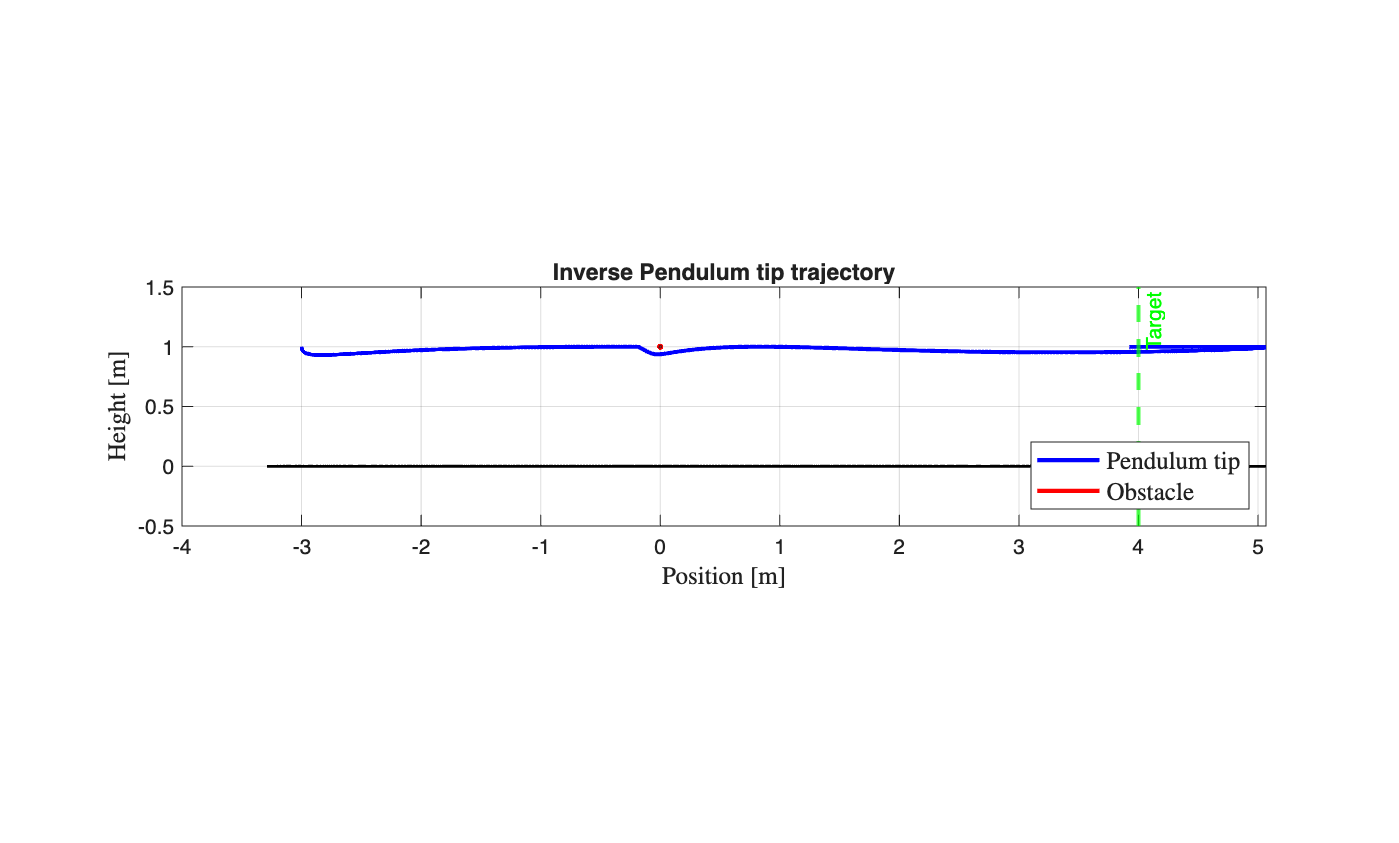
\includegraphics[width=\textwidth]{INF/Fig2_rk_inf_2.png}
		\end{subfigure}
	\end{figure}
\end{frame}	

	\begin{frame}{Risultati Simulazione - Set 3 - INF}
	\begin{figure}
		\centering
		\begin{subfigure}[b]{0.48\textwidth}
			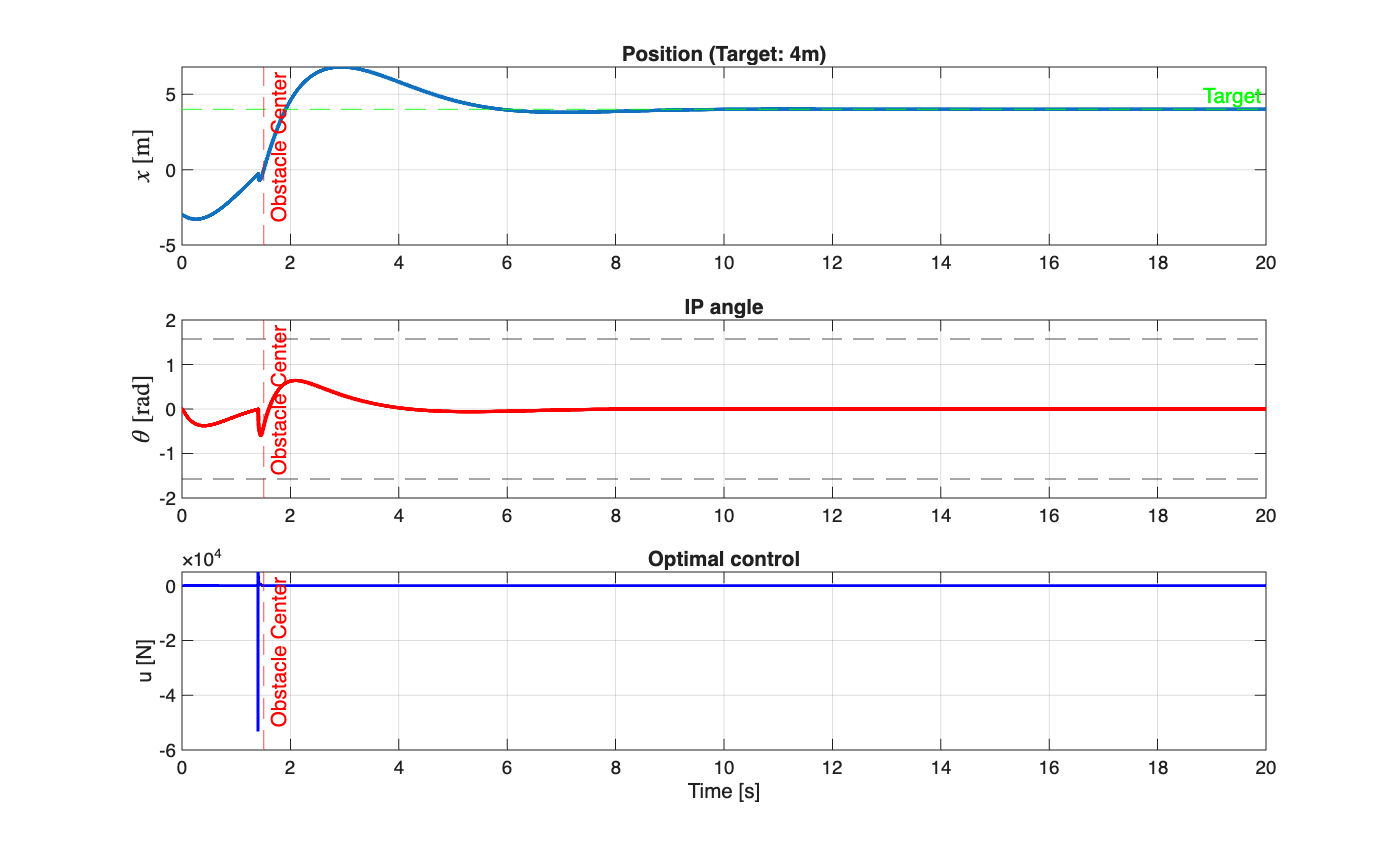
\includegraphics[width=\textwidth]{INF/Fig1_eu_inf_3.png}
			
		\end{subfigure}
		\hfill
		\begin{subfigure}[b]{0.48\textwidth}
			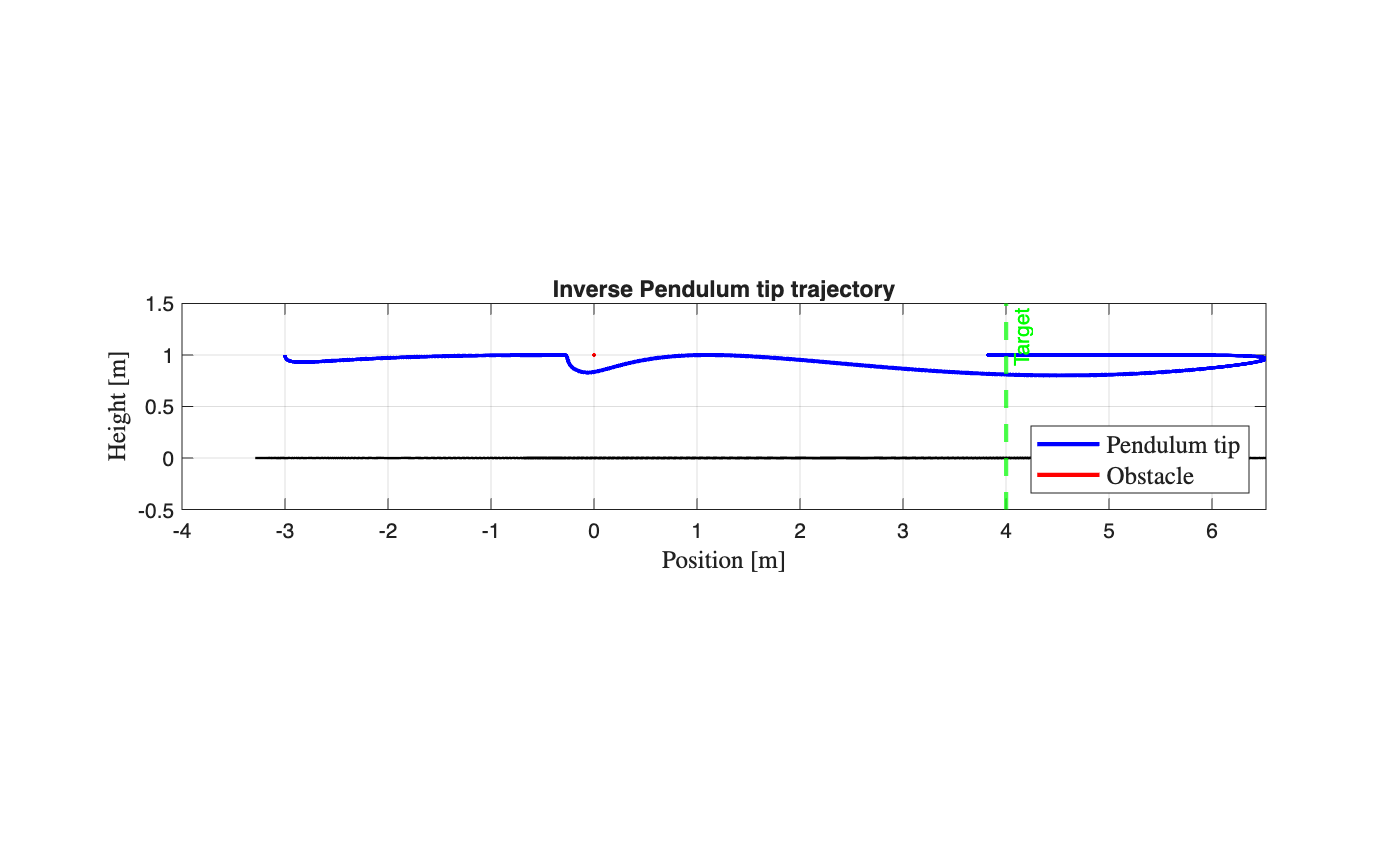
\includegraphics[width=\textwidth]{INF/Fig2_eu_inf_3.png}
			
		\end{subfigure}
		
		\vspace{0.2cm}
		
		\begin{subfigure}[b]{0.48\textwidth}
			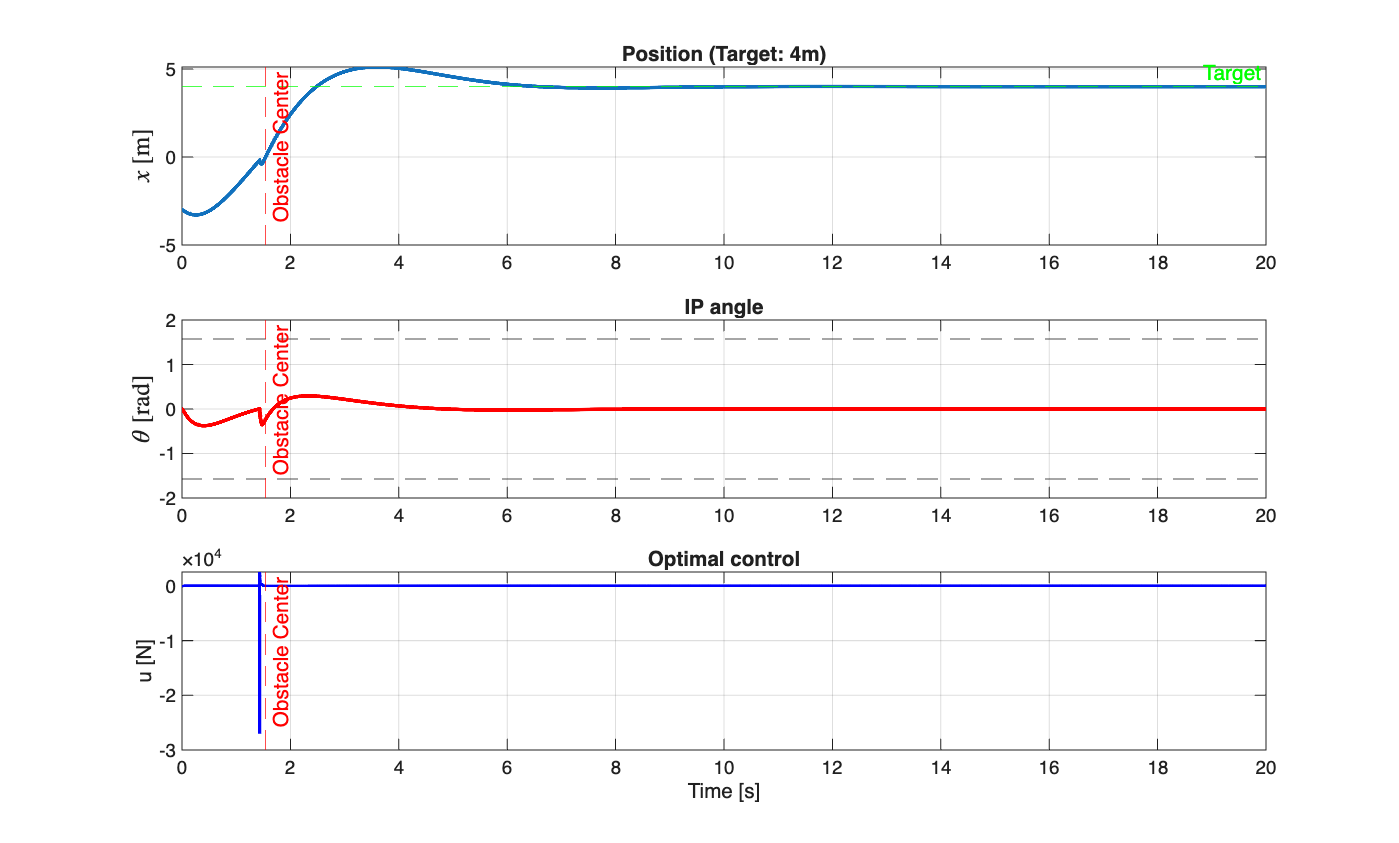
\includegraphics[width=\textwidth]{INF/Fig1_rk_inf_3.png}
		\end{subfigure}
		\hfill
		\begin{subfigure}[b]{0.48\textwidth}
			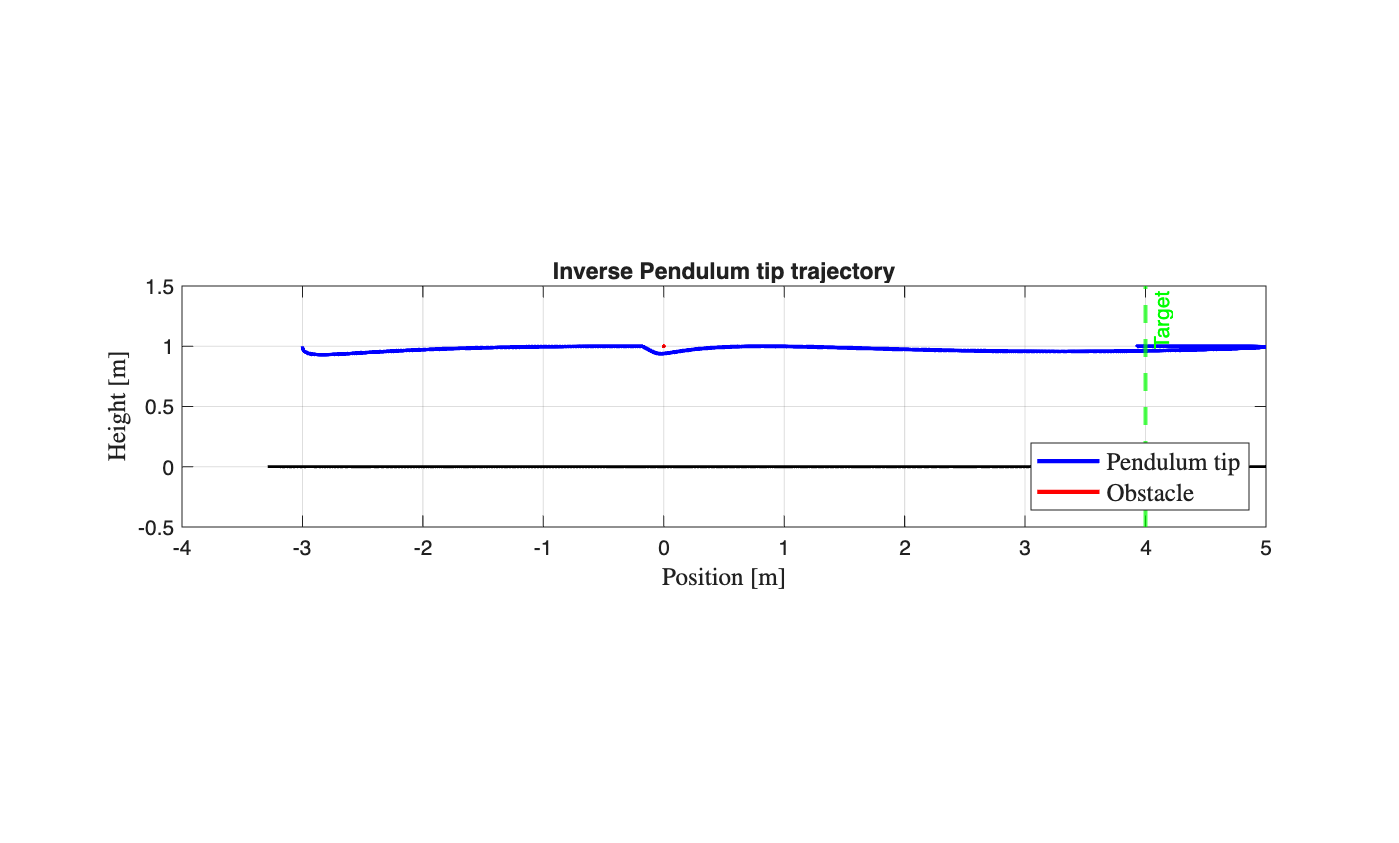
\includegraphics[width=\textwidth]{INF/Fig2_rk_inf_3.png}
		\end{subfigure}
	\end{figure}
\end{frame}	

	\begin{frame}{Risultati Simulazione - Set 4 - INF}
	\begin{figure}
		\centering
		\begin{subfigure}[b]{0.48\textwidth}
			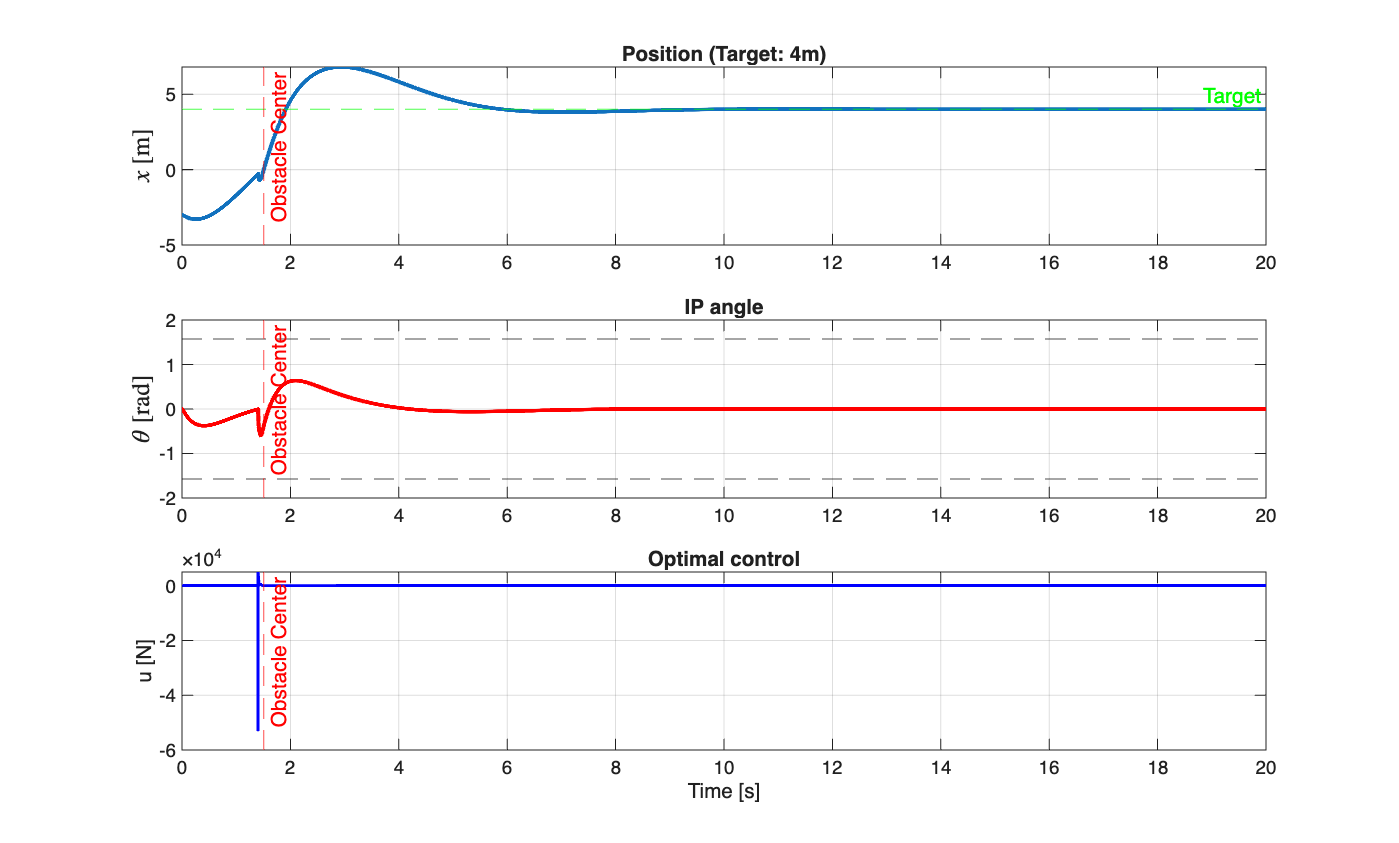
\includegraphics[width=\textwidth]{INF/Fig1_eu_inf_4.png}
			
		\end{subfigure}
		\hfill
		\begin{subfigure}[b]{0.48\textwidth}
			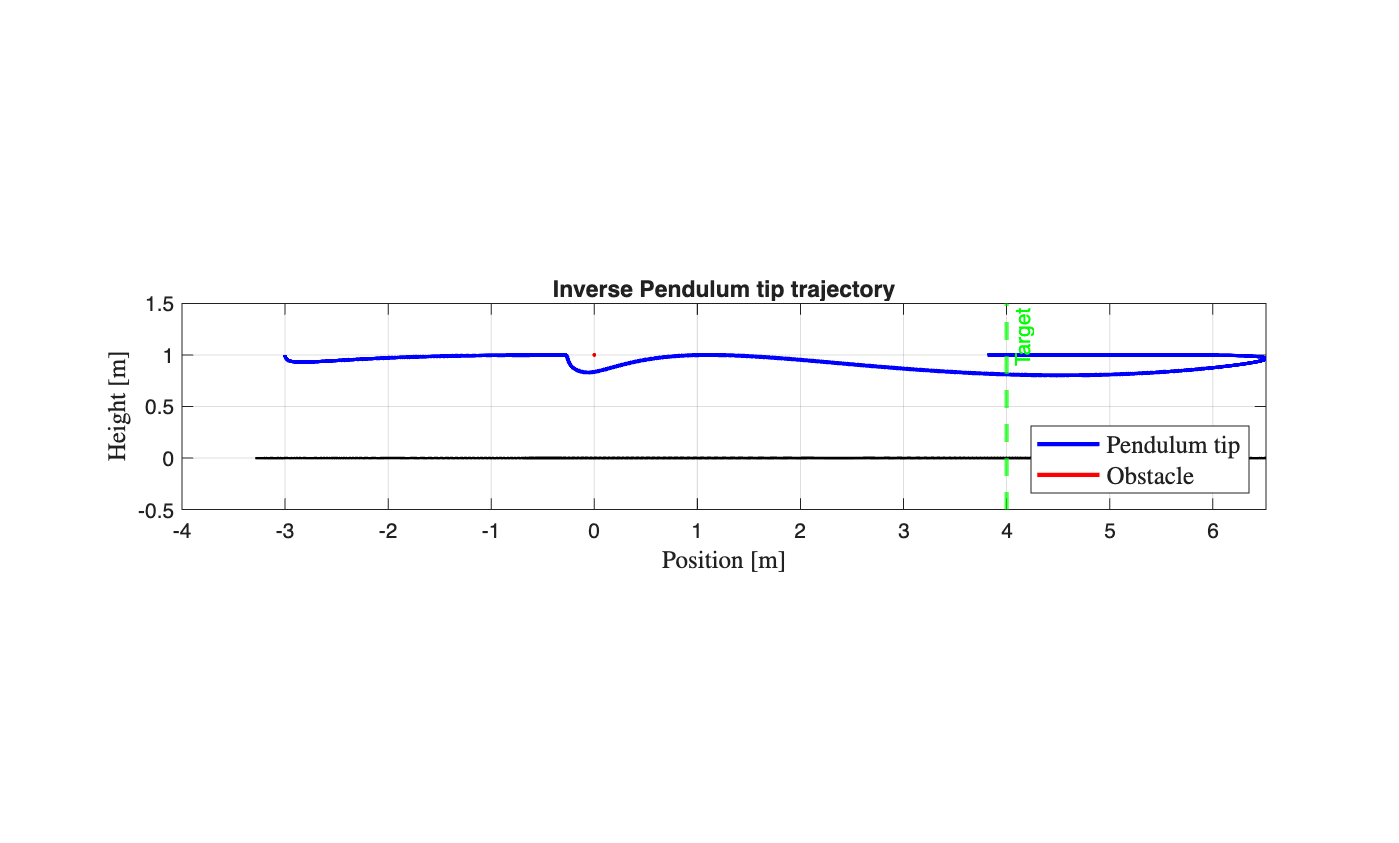
\includegraphics[width=\textwidth]{INF/Fig2_eu_inf_4.png}
			
		\end{subfigure}
		
		\vspace{0.2cm}
		
		\begin{subfigure}[b]{0.48\textwidth}
			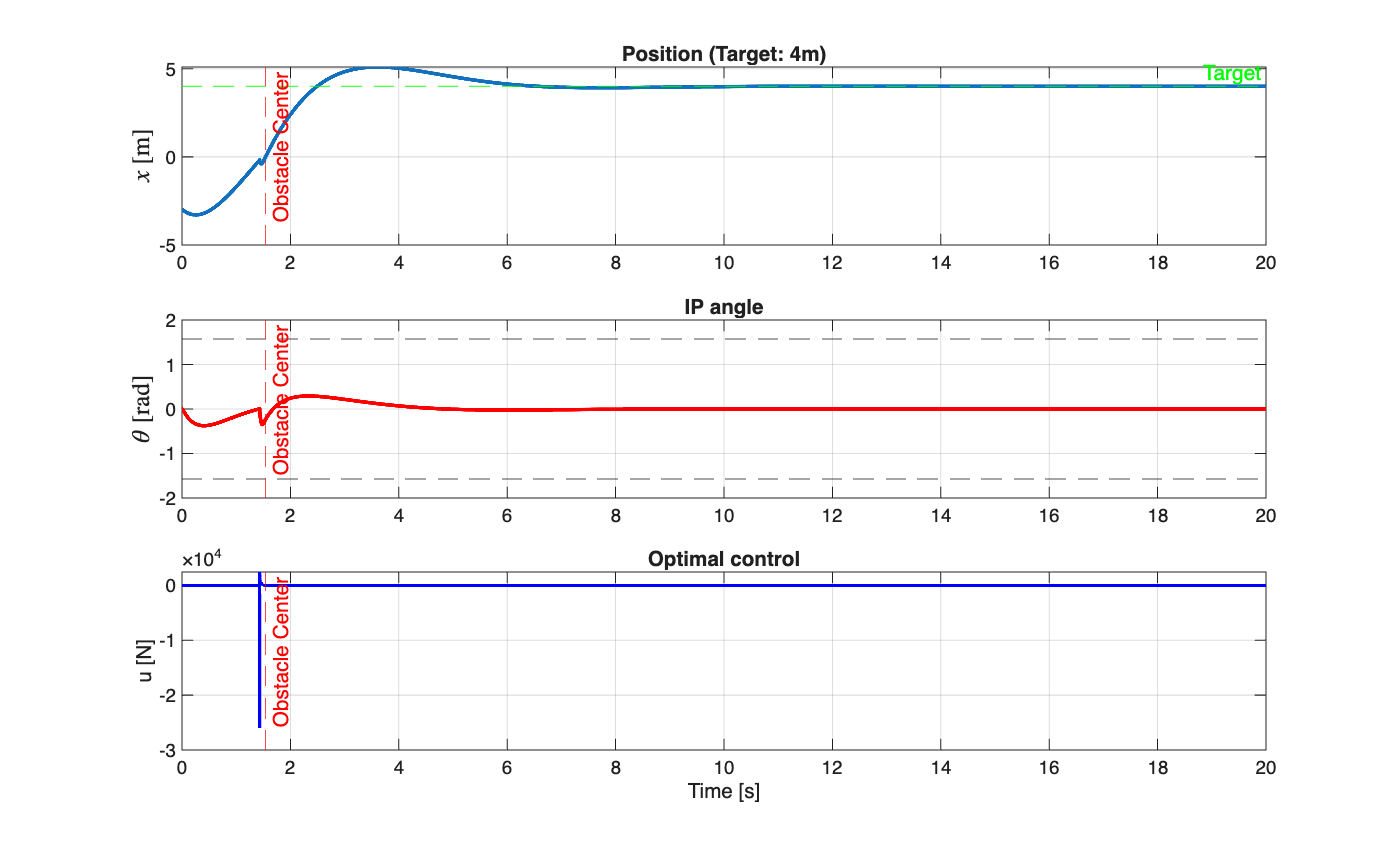
\includegraphics[width=\textwidth]{INF/Fig1_rk_inf_4.png}
		\end{subfigure}
		\hfill
		\begin{subfigure}[b]{0.48\textwidth}
			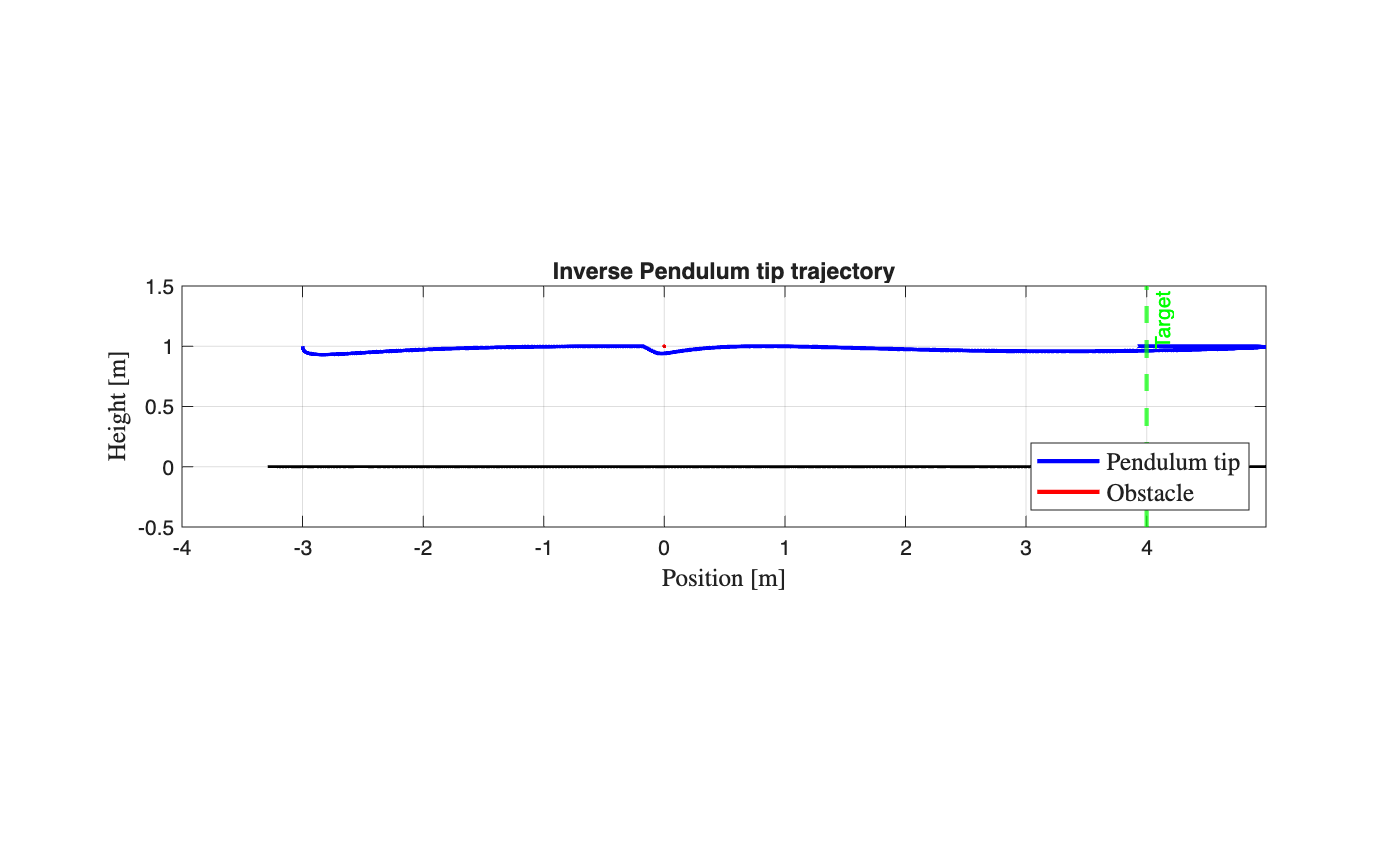
\includegraphics[width=\textwidth]{INF/Fig2_rk_inf_4.png}
		\end{subfigure}
	\end{figure}
\end{frame}	



	
\end{document}